% 每个提纲下直接填写正文；长度增加时自动续页并重复版框。
\CasmTopic{1. 课题的立项依据}{（研究意义、国内外研究现状及发展动态分析，附主要参考文献目录）\\
（小四号字体，中文字体为宋体，英文字体为Times New Roman，1.25 倍行距）}

% 内容来源：NSFC_2027_Mapping/extraTex/1.1.立项依据.tex
\subsection*{1.1\quad 研究背景与意义}

对地观测数据的规模增长已经远远超过人工判读能力。在资源调查、国土监测、灾害应急等业务中，使用者真正需要的往往不是“某一景影像的编号”，而是“哪些影像里出现了某种地物组合与空间格局”。以自然语言直接检索遥感影像，因此成为把海量影像库转化为可用地理信息的一条关键途径：它不要求使用者预先掌握波段、传感器与产品级别等专业参数，也不受固定类别体系的限制，允许用一句自然描述表达带有空间关系的复合需求，例如“河流两侧分布着成排厂房”。 上述检索需求与描述覆盖不足之间的矛盾见图~\ref{fig:background}。

% F1: F01_研究背景与问题提出-v4.png
\begin{figure}[!htbp]
    \centering
    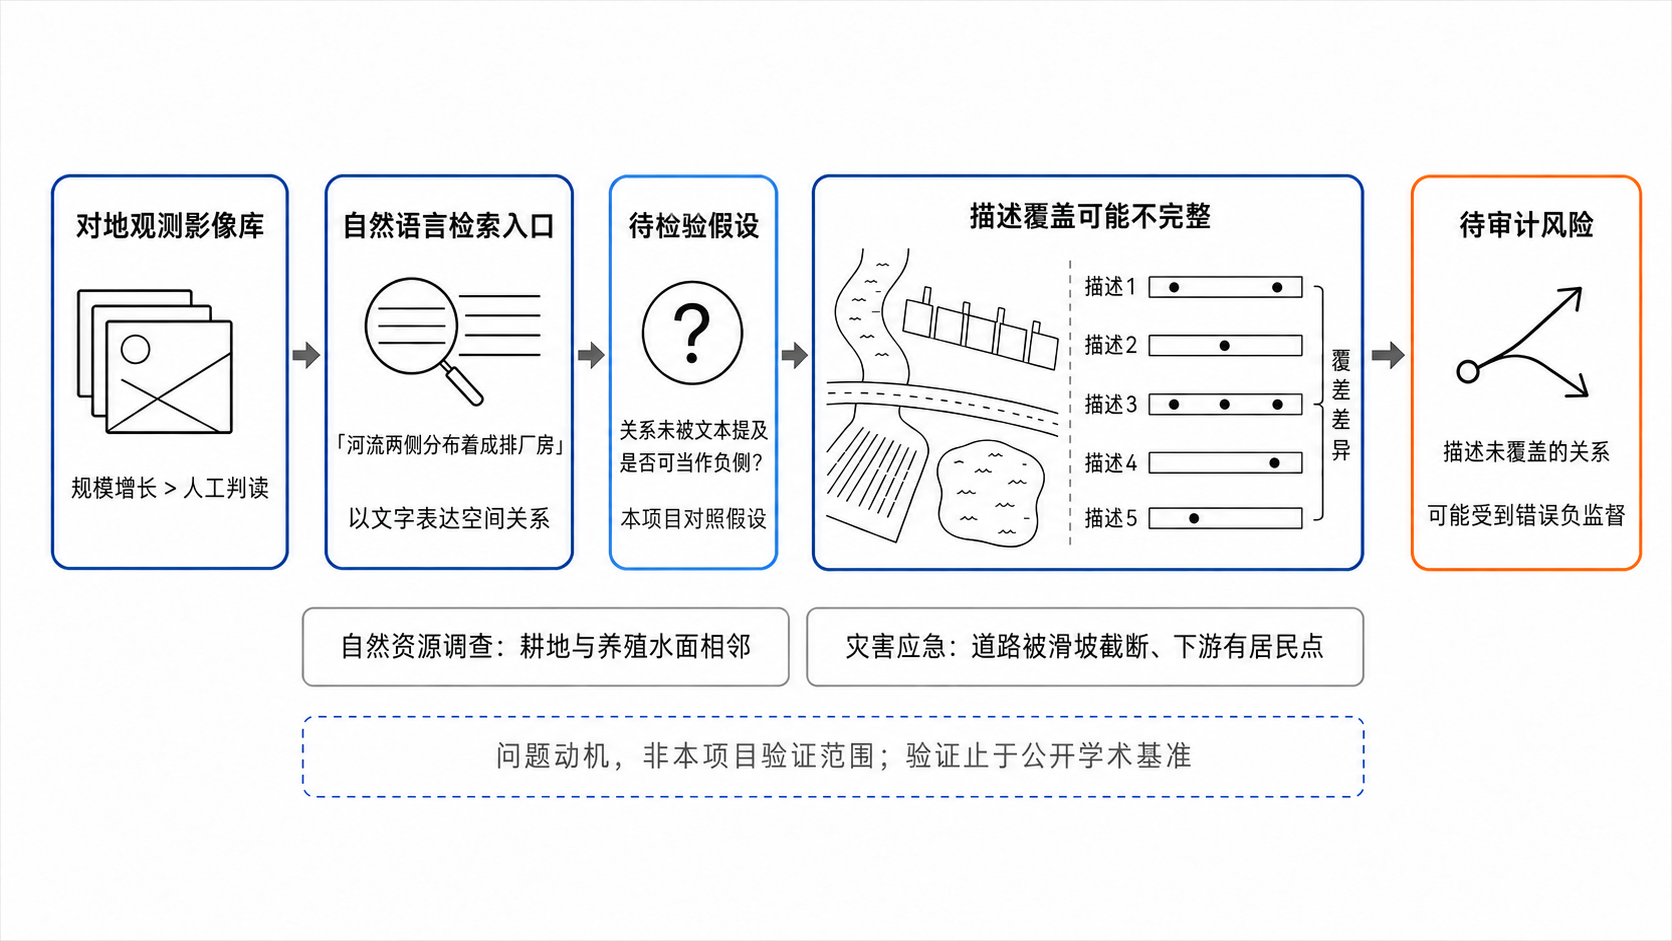
\includegraphics[trim=32bp 125bp 11bp 156bp,clip,width=\linewidth]{figures/F01_研究背景与问题提出-v4.png}
    \caption{研究背景与问题提出。业务场景用于说明研究动机，项目验证范围为公开学术基准。}
    \label{fig:background}
\end{figure}


围绕这一目标，遥感图文检索在近年形成了相对完整的研究体系。国内学者从多模态对齐的角度系统梳理了遥感领域时空对齐与语义对齐的发展脉络\cite{lishutao2025alignment}，并对遥感场景下图文跨模态理解的任务划分、公开数据与评价指标做了归纳\cite{zhengxiangtao2025crossmodal}；面向图文检索这一具体任务，视觉语言基础模型驱动下的研究进展也已被专门综述\cite{wuhui2026rsitr}。国际上，遥感视觉语言模型的能力边界与发展趋势同样得到系统评述\cite{li2024vlmrsmag}，并出现了对检索方法与数据基础演化的横向对比\cite{rsitrreview2025}。

自然语言描述对影像内容的覆盖程度，会影响图文匹配的监督含义。一景遥感影像通常同时包含道路、建筑、水体、植被及其空间格局，一条人工描述往往只涉及其中一部分。RSITMD 强调细粒度、低冗余描述，每图配置 5 条描述并附关键词\cite{yuan2022amfmn}。RSICD 虽也保留每图 5 条记录，但原论文说明仅 724 幅影像具有 5 条不同描述，4853 幅只有 1 条，不足部分由已有句子复制补齐\cite{lu2018rsicd}。因此，记录条数不能代表独立证据量；描述是否互补及其覆盖差异，必须在去重和来源核对后审计。

描述的不完备使关系监督面临歧义：文本没有提及某一关系，既不能证明该关系存在，也不能证明其与影像冲突。如果据此构造关系负例，就可能引入缺乏依据的惩罚。\textbf{如何区分有视觉证据的关系冲突与尚不可判定的关系，并据此构造跨模态匹配中的关系监督，是本项目要回答的问题。}地物之间的相邻、包含、方位与距离关系常用于表达复合检索需求，也可能在简短描述中被省略。图~\ref{fig:three-state}示意不同证据状态及其监督处理方式。

% F2: F02_三态歧义-v2.png
% 与正文共页，避免该图单独占据浮动页。
\begin{figure}[!htb]
    \centering
    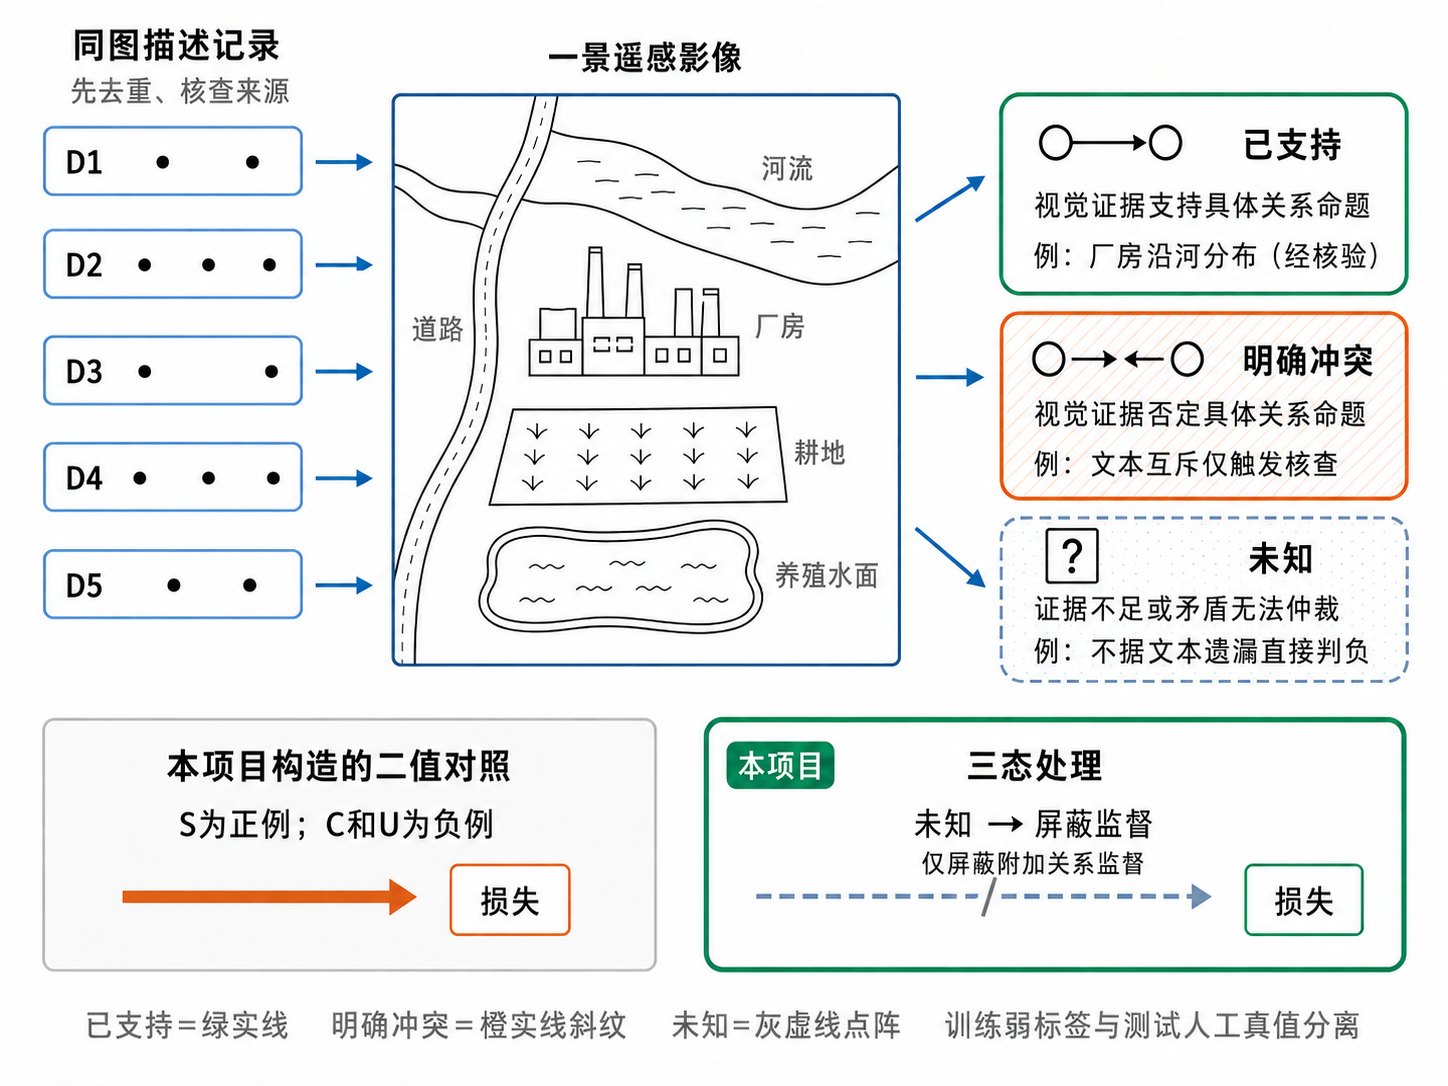
\includegraphics[width=0.90\linewidth]{figures/F02_三态歧义-v2.png}
    \caption{描述不完备导致的三态歧义。未提及与明确冲突分开判定；未知关系不参与监督。}
    \label{fig:three-state}
\end{figure}


这一问题的现实分量可以从典型业务场景看出。在自然资源调查中，作业人员需要从历史影像库中找出“耕地与养殖水面相邻”的地块以核查用途变化；在灾害应急中，需要快速定位“道路被滑坡体截断、下游有居民点”的区域。这些需求的共同点是：检索意图由\textbf{地物及其空间关系}共同定义，而非单个地物类别。也正因如此，检索系统对关系的处理方式直接决定其可用性——把“文本没提到水体”理解为“影像里不应有水体”，会让大量本应召回的影像被排除；反过来，若对关系一概不作约束，“建筑在道路左侧”与“建筑在道路右侧”就无法区分。

项目验证范围限定为 RSITMD、RSICD 及其关系挑战子集。业务场景用于说明研究动机，公开基准结论向实际作业推广仍需检验数据域差异、精度和作业规范适配。

本项目的科学价值在于检验关系证据状态如何影响监督构造，并给出可复核的表示、学习与验证方式。应用价值体现在结果解释：区分被影像证据否定的关系与暂时无法判定的关系，为后续人工核查提供依据。

\subsection*{1.2\quad 国内外研究现状及发展动态分析}

\subsubsection*{1.2.1\quad 任务基准与评测口径}

遥感图文检索的基准体系以 RSICD\cite{lu2018rsicd} 与 RSITMD\cite{yuan2022amfmn} 为核心，评测普遍采用双向 R@1/R@5/R@10 及六项均值 mR。近年出现了规模更大、语义更丰富的数据资源：SkyScript 将影像与开放地理数据的语义相连接\cite{wang2024skyscript}，RS5M 构建了大规模遥感图文数据并训练了相应模型\cite{zhang2024rs5m}，LuoJiaHOG 则从层次化、地理感知的角度组织图像描述\cite{zhao2025luojiahog}。综述工作指出，早期数据集场景较简单、描述较短，后期数据集才引入复杂场景与细粒度描述，而更新的大规模数据集多依赖自动或半自动生成描述以扩充语义多样性\cite{rsitrreview2025}。这一演化在扩大数据规模的同时，也把描述质量与覆盖程度的不确定性引入了训练与评测。

\subsubsection*{1.2.2\quad 跨模态对齐方法的演进}

方法研究的主线是让图文对齐“更细”。通用图文匹配领域的堆叠交叉注意力\cite{lee2018scan}、相似度推理与过滤\cite{diao2021sgraf} 与可插拔匹配调节机制\cite{diao2023regulator} 奠定了细粒度交互范式。遥感场景中，从语义对齐网络\cite{cheng2021dsan}、细粒度多尺度适配\cite{yuan2022amfmn} 到全局与局部信息结合\cite{yuan2022galr}，再到基于 Transformer 的文本到影像检索\cite{rahhal2022multilanguage}、多任务引导融合编码\cite{fusionencoder2023}、先验指令表示\cite{pan2023pir}、全局—局部软对齐\cite{zhang2024glisa} 与多尺度语义感知\cite{mssa2025}，构成了一条持续细化的技术脉络。最近的工作开始关注遥感数据自身的分布特点：模内相似度显著高于自然图像使正负样本难以区分，因此引入负样本扩展与分布匹配约束\cite{dcca2026}，以及面向类别中心漂移的语义对齐\cite{cglsa2026}。与此并行，参数高效迁移\cite{yuan2023peft} 与提示学习\cite{zhou2022cocoop} 使有限算力下适配大模型成为常规做法。

这些方法提高了图文对齐的细粒度，但标准配对目标本身不能说明非配对影像是否满足某一具体关系命题；这一问题需要额外的关系证据和专门评测。

\subsubsection*{1.2.3\quad 视觉语言基础模型改变了研究起点}

CLIP 及其大规模图文对比预训练范式\cite{radford2021clip} 之后，遥感领域相继出现了 RemoteCLIP\cite{liu2024remoteclip}、GeoRSCLIP\cite{zhang2024rs5m} 与多模态遥感基础模型 SkySense\cite{guo2024skysense}。这些工作把研究起点从“从零设计双塔”推进到“在强预训练模型上做领域适配”。综述同时指出，通用视觉语言模型在遥感等特殊领域常因分布差异导致性能显著下降\cite{li2024vlmrsmag,wuhui2026rsitr}，因此领域适配而非从零训练成为务实选择。有一点必须点明：RemoteCLIP 的训练使用了与检索基准相关的数据\cite{liu2024remoteclip}，这意味着它在这些基准上的结果不能被表述为严格意义上的零样本泛化——这一点直接影响后续比较的有效性。

\subsubsection*{1.2.4\quad 实体与空间关系已被引入}

把地理实体与空间关系引入遥感图文检索并非新设想。已有研究从单模态角度探索实体与关系的特征学习以缓解信息冗余\cite{zhang2023unimodal}，也有工作通过伪区域与空间—通道注意力刻画目标的空间分布\cite{wu2024scat}，或以方向为导向构建视觉语义嵌入\cite{yang2024dove}，还有工作引入外部知识增强检索\cite{mi2024knowledgeaware}；面向遥感图文检索的空间感知实体关系探索也已发表\cite{shui2025esrn}。通用领域则有基于场景图的图文检索融合\cite{sgfn2023} 与实例间语义关系学习\cite{pan2023semrel}。\textbf{因此，“引入空间关系”本身已是成熟方向，本项目不以此为创新主张。}

与此同时，视觉语言模型在组合性与空间推理上的系统性弱点在自然图像上已有证据：Winoground 揭示了模型在组合语义上的困难\cite{thrush2022winoground}，视觉空间推理基准显示空间关系理解仍是薄弱环节\cite{liu2023vsr}。这些结论来自自然图像，能否外推到遥感影像仍需在遥感基准上重新检验——遥感影像的方位关系还受成像坐标系与几何增强影响，不能直接照搬。

关系语义可以通过大规模预训练隐式学习\cite{liu2024remoteclip,zhang2024rs5m,guo2024skysense}，也可以通过关系结构显式增强\cite{zhang2023unimodal,wu2024scat,shui2025esrn}。本项目关注两条路径共同面对的监督问题：当数据只提供图像级描述时，如何为具体关系命题确定可用的正、负证据，并保留不能判定的状态。描述不完备造成多大影响，以及三态处理是否带来收益，均需由审计与对照检验。

\subsubsection*{1.2.5\quad 图文对应中的噪声与弱对齐}

图文对不完全匹配的问题已有系统研究：部分错配对的鲁棒学习\cite{hu2023rcl}、基于元学习的相似度校正\cite{han2023msc}、双向相似度一致性纠正\cite{yang2023bicro}、证据深度学习处理噪声对应\cite{qin2022decl}、负样本预感知\cite{zhang2024npc} 与三分法处理\cite{feng2024tripartition} 构成了较完整的方法谱系。在遥感领域，PMPGuard 针对“伪匹配对”提出了跨模态门控注意力与正负感知注意力，并在合成失配率与真实数据上做了验证\cite{pmpguard2026}。

这些方法并非都把失配统一视为无用噪声。PMPGuard 通过匹配程度估计与注意力机制，区分并利用部分匹配图文中的正、负语义线索\cite{pmpguard2026}。其启发在于保留有效语义；本项目进一步检验具体“影像—实体对—关系命题”的支持、冲突与未知状态如何参与监督。训练数据构造也会影响鲁棒性\cite{nguyen2022quality}，自动采集与过滤的大规模图文数据\cite{schuhmann2022laion}尤其需要区分标注错误、内容遗漏与视觉不可判定三种情形。

\subsubsection*{1.2.6\quad 国内研究力量与进展}

国内团队在该方向具有较强的研究基础与体系化推进。在数据与基准层面，RSICD\cite{lu2018rsicd} 与 RSITMD\cite{yuan2022amfmn} 两个被国际广泛使用的遥感图文基准均由国内团队构建，LuoJiaHOG\cite{zhao2025luojiahog} 进一步引入层次化与地理感知的描述组织方式。在方法层面，从全局与局部信息结合\cite{yuan2022galr}、实体与关系的单模态特征学习\cite{zhang2023unimodal}、先验指令表示\cite{pan2023pir}，到空间--通道注意力\cite{wu2024scat}、全局--局部软对齐\cite{zhang2024glisa} 与空间感知实体关系探索\cite{shui2025esrn}，国内工作构成了该方向的主要推进力量。在综述与方向研判层面，多模态对齐的挑战与机遇\cite{lishutao2025alignment}、遥感场景图文跨模态理解的任务划分\cite{zhengxiangtao2025crossmodal} 以及视觉语言基础模型驱动的图文检索进展\cite{wuhui2026rsitr} 相继发表，为该领域提供了系统的问题梳理。

换言之，这是一个国内力量密集、竞争充分的方向。本项目因此不以“补国内空白”为定位；要找的是在这样一个成熟方向上仍未被正面处理的建模前提问题。 三条研究脉络与本项目切入点的关系见图~\ref{fig:landscape}。

% F3: F03_研究现状与切入点-v3.png
\begin{figure}[!htbp]
    \centering
    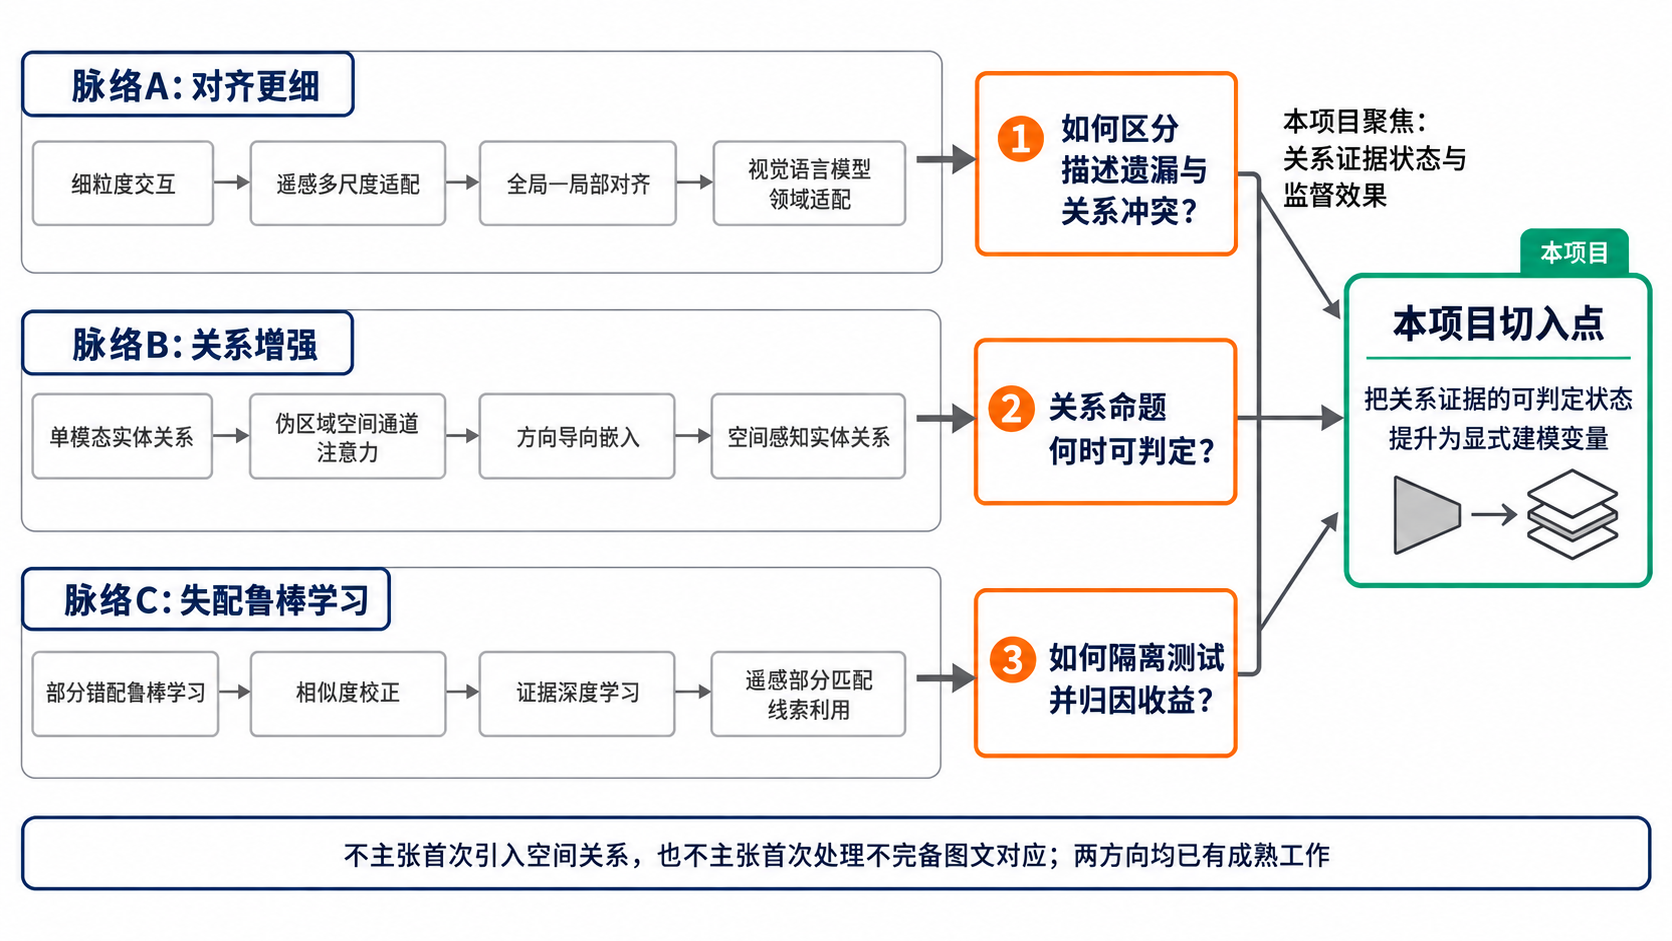
\includegraphics[width=\linewidth]{figures/F03_研究现状与切入点-v3.png}
    \caption{研究现状与本项目切入点。关系增强与失配处理已有研究基础，本项目关注关系证据的可判定状态。}
    \label{fig:landscape}
\end{figure}


\subsection*{1.3\quad 现有研究的不足}

上述工作为关系增强和失配处理提供了基础。本项目在此基础上检验以下三个相互关联的问题，重点是具体关系命题的证据状态、监督构造与验证边界。

\begin{enumerate}
    \item 描述遗漏与关系冲突对监督的影响需要分别检验。已有研究从鲁棒学习、相似度校正、样本划分及有效语义保留等角度处理失配\cite{hu2023rcl,han2023msc,yang2023bicro,zhang2024npc,feng2024tripartition,pmpguard2026}。本项目关注其中更具体的情形：当描述没有覆盖某关系时，能否获得支持或冲突的视觉证据\cite{lu2018rsicd,yuan2022amfmn}；若不能，增加关系负例约束是否反而损害匹配。

    \item 关系表示还需要与证据可信度共同考察。已有实体与空间关系研究关注关系特征与对齐\cite{zhang2023unimodal,shui2025esrn,wu2024scat,yang2024dove,mi2024knowledgeaware}，但图像级描述本身不提供实体框、关系图或拓扑真值。自动抽取的三元组只能作为弱监督；其对应命题在影像中是否成立，仍需视觉判定。对全文尚未取得的工作，本项目只依据可核验题录说明研究主题，不据此断言其缺少某种状态建模。

    \item 评测口径难以支撑可归因的结论。 综述已指出跨论文数字因协议差异而难以统一比较\cite{rsitrreview2025}；同时，预训练数据与检索基准之间存在重叠\cite{liu2024remoteclip}，大规模数据集又普遍依赖自动生成描述\cite{rsitrreview2025,zhang2024rs5m}。在缺少近重复去重与分层报告的情况下，性能提升可能来自骨干容量、训练预算或数据泄漏，而非所声称的机制。
\end{enumerate}

\subsection*{1.4\quad 关键科学问题与研究切入点}

\subsubsection*{1.4.1\quad 关键科学问题}

本项目拟解决的关键科学问题是：

\begin{quote}
\textbf{在遥感图文数据中文本描述对影像内容的覆盖天然不完备的条件下，如何在跨模态匹配中区分“描述未覆盖”与“实际关系冲突”，使有证据的地理实体关系参与约束、而不可判定的关系不被当作监督信号？}
\end{quote}

围绕这一问题，形成三个相互支撑的子问题：（1）\textbf{表示层}，如何构建带证据与置信度的实体—关系记录，使“已支持、明确冲突、未知”三态可判定、可人工复核；（2）\textbf{学习层}，三态信息以何种方式进入对齐或重排序目标，才能在不牺牲标准配对召回的前提下降低关系冲突导致的误匹配；（3）\textbf{验证层}，如何构造评测协议，使性能变化可归因于关系建模本身，而非骨干容量、训练预算或数据泄漏。

问题的可检验性在于：可核验的关系证据是否改变监督信号的效果。项目先审计描述遗漏相关错误是否具有足够比例，再比较忽略关系、未知作负例与未知屏蔽三种处理，并控制模型和训练预算。若审计不支持现象的重要性，或等预算对照不支持三态处理的收益，则相应假说不成立，研究结论据此收缩。

\subsubsection*{1.4.2\quad 研究思路与拟检验的假说}

本项目以具体关系命题的可判定状态为切入点。先对同图描述去重并核对来源，将覆盖差异作为弱线索，再结合视觉证据区分支持、冲突与未知；在已有视觉语言编码器上研究可核验关系的监督作用，并用标准检索和独立关系挑战评测检验效果。

据此提出三条可证伪假说。\textbf{H1（现象存在性）}：在固定基线的检索错误审计中，能稳定识别“候选影像支持查询关系、但其配对描述未覆盖该关系”的情形，其占比达到预设的 10\% 继续投入阈值。\textbf{H2（机制判断）}：相较于将未知关系作为负例，三态区分与未知屏蔽能够降低关系冲突误匹配率，且支持返回率不降低、未知返回率不增加、标准检索 mR 的绝对下降不超过 1 个百分点。\textbf{H3（可归因性）}：上述改善在等参数量、等训练步数和固定数据划分下仍然成立，不能仅由容量、预算或数据重叠解释。

H1 在启动阶段（2026 年 11 月至 2027 年 1 月）检验：从 600 组验证集审计影像中，每图按固定规则选择 1 条描述查询，以固定基线在验证图库中的 top-1 非原配返回数为分母；双人核验返回影像是否支持查询中明确的关系命题，并核对该候选的去重配对描述是否均未提及该关系。满足两项条件者计入分子；无关系命题或视觉不可判定者保留在分母并另报数量。该比例是描述遗漏相关现象的操作性指标，不单凭它认定错误的因果来源。分别报告两个基准及合并比例与 Wilson 95\% 置信区间；若没有基线错误则记为不可估计。\textbf{10\% 为预先确定的研究取舍阈值。}区间上限低于阈值，或归因不能稳定复核时，研究重点收缩为关系冲突识别；跨越阈值时保留不确定结论。

\subsubsection*{1.4.3\quad 预期贡献}

本项目预期形成三方面贡献：在\textbf{问题层面}，量化描述遗漏相关情形并给出具体关系命题的三态判定规范；在\textbf{方法层面}，比较忽略关系、未知作负例与未知屏蔽的效果边界；在\textbf{评测层面}，形成包含候选真值核验、未知态报告、近重复去重与等预算对照的独立验证协议。

需要说明的是，本项目\textbf{不主张}首次引入空间关系或首次处理不完备图文对应——如前所述，这两个方向均已有成熟工作。本项目主张的是对关系证据状态的显式区分及其在监督信号构造中的作用，这是一个方法层面的问题重述与验证设计。

% 文献目录由 references/myexample.bib 自动生成。
\MappingBibliography


\CasmTopic{2. 课题的研究内容、研究目标，以及拟解决的关键科学问题}{（此部分为重点阐述内容）}

% 内容来源：NSFC_2027_Mapping/extraTex/2.1.研究内容.tex
\subsection*{2.1\quad 研究目标}

\textbf{总体目标}：建立面向不完备文本描述的地理实体关系证据表示与跨模态匹配方法，形成可复现的分层评测协议，使遥感图文检索在关系敏感场景下的失效模式可识别、可缓解、可归因。

三个具体目标与后文研究内容一一对应：

\begin{enumerate}
    \item 目标一（表示）：完成 RSITMD 与 RSICD 各 300 组、合计 600 组影像及其全部描述的审计，形成不超过 20 类实体、10 类关系的词表与三态判定规范各 1 套；计划交付 1800 条人工核验关系挑战记录，全部经双人独立标注，以仲裁前三态标注一致性 Cohen's $\kappa \geq 0.70$ 为质量目标。
    \item 目标二（学习）：形成仅约束可核验关系、屏蔽未知态的匹配方法与训练推理代码 1 套。完成 3 个处理臂在 2 个基准、3 个随机种子下的 18 次主实验；性能验证目标为相对“未知作负例”臂降低关系冲突误匹配率、保持支持返回率不降低，并将两个基准上标准 mR 的绝对降幅分别控制在 1 个百分点以内，按预先确定的置信区间判据报告是否达到目标。
    \item 目标三（验证）：形成标准检索、关系挑战、覆盖度、迁移和效率五类评测报告及协议 1 套，完成 12 次关键消融实验，形成至少 3 个随机种子的等预算对照证据；交付可复现材料和轻量检索演示各 1 套，完成 1 篇论文并投稿，提交结题研究报告 1 份。
\end{enumerate}

图~\ref{fig:framework}给出三个目标对应的研究内容、交付物及错误归因回流关系。

% F4: F04_总体框架-v3.png
\begin{figure}[!htbp]
    \centering
    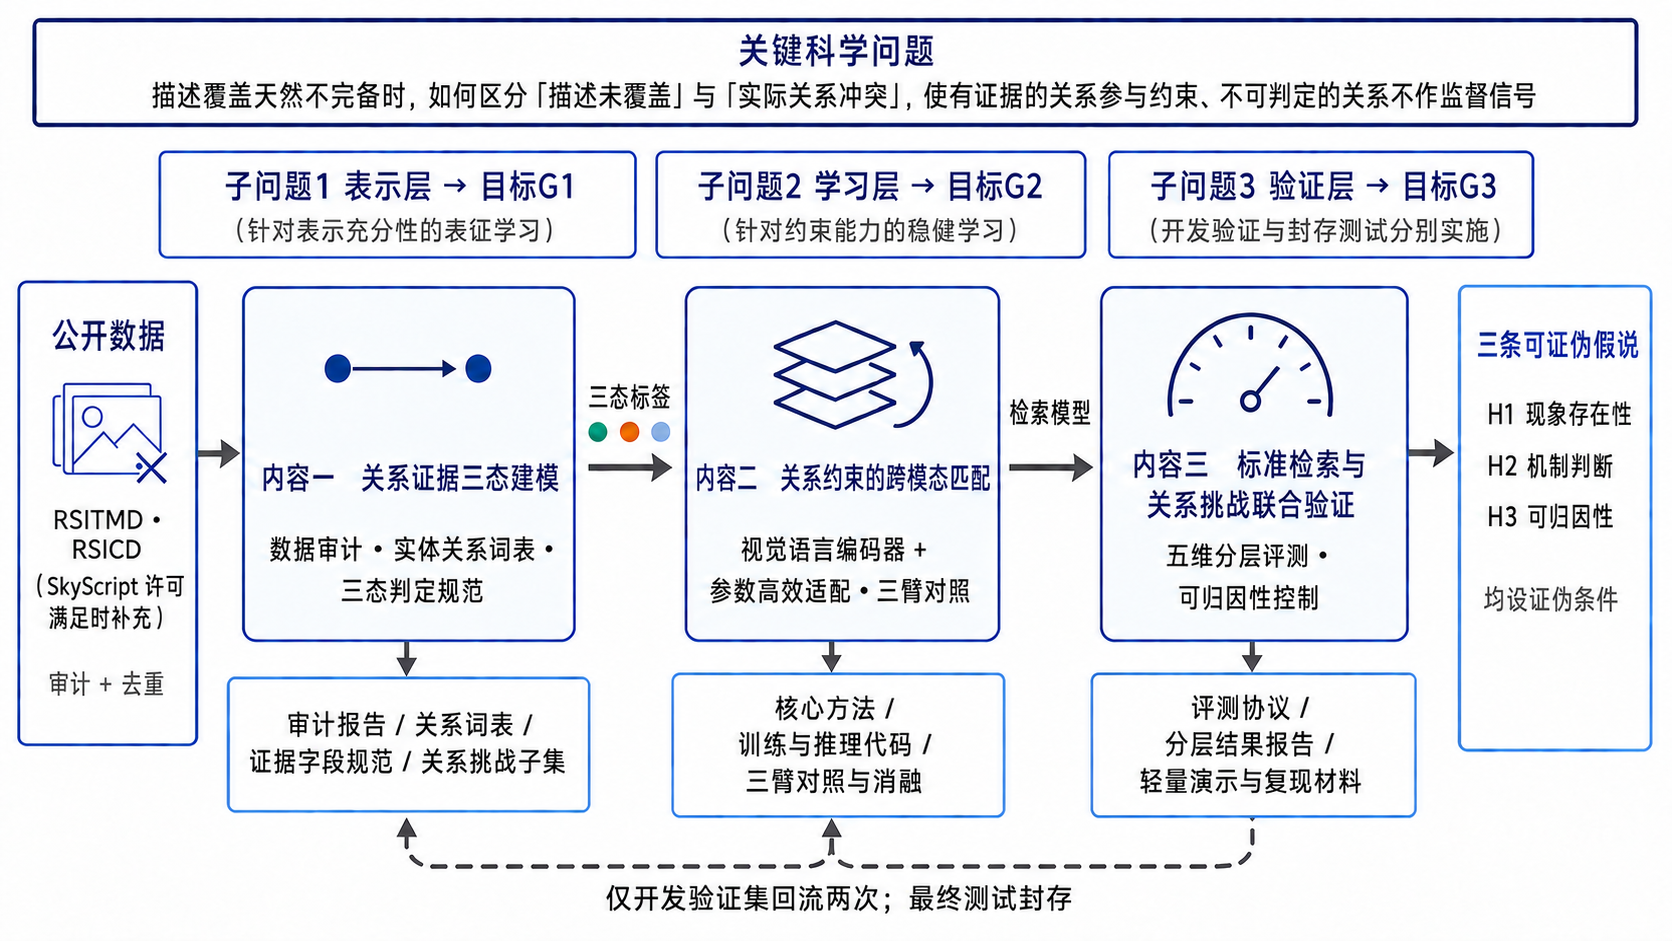
\includegraphics[width=\linewidth]{figures/F04_总体框架-v3.png}
    \caption{总体研究框架。回流仅使用开发与验证数据；最终测试在规范、方法与参数冻结后一次性实施。}
    \label{fig:framework}
\end{figure}

\subsection*{2.2\quad 研究内容}

\subsubsection*{2.2.1\quad 内容一：不完备描述条件下的地理实体关系证据建模}

本内容回答“关系证据的三态如何可判、可复核地表示”。 具体技术路线见图~\ref{fig:route-one}。

% F5: F05_技术路线一-v3.png
% 与后续正文合排，避免生成上下大幅留白的独立插图页。
\begin{figure}[!htb]
    \centering
    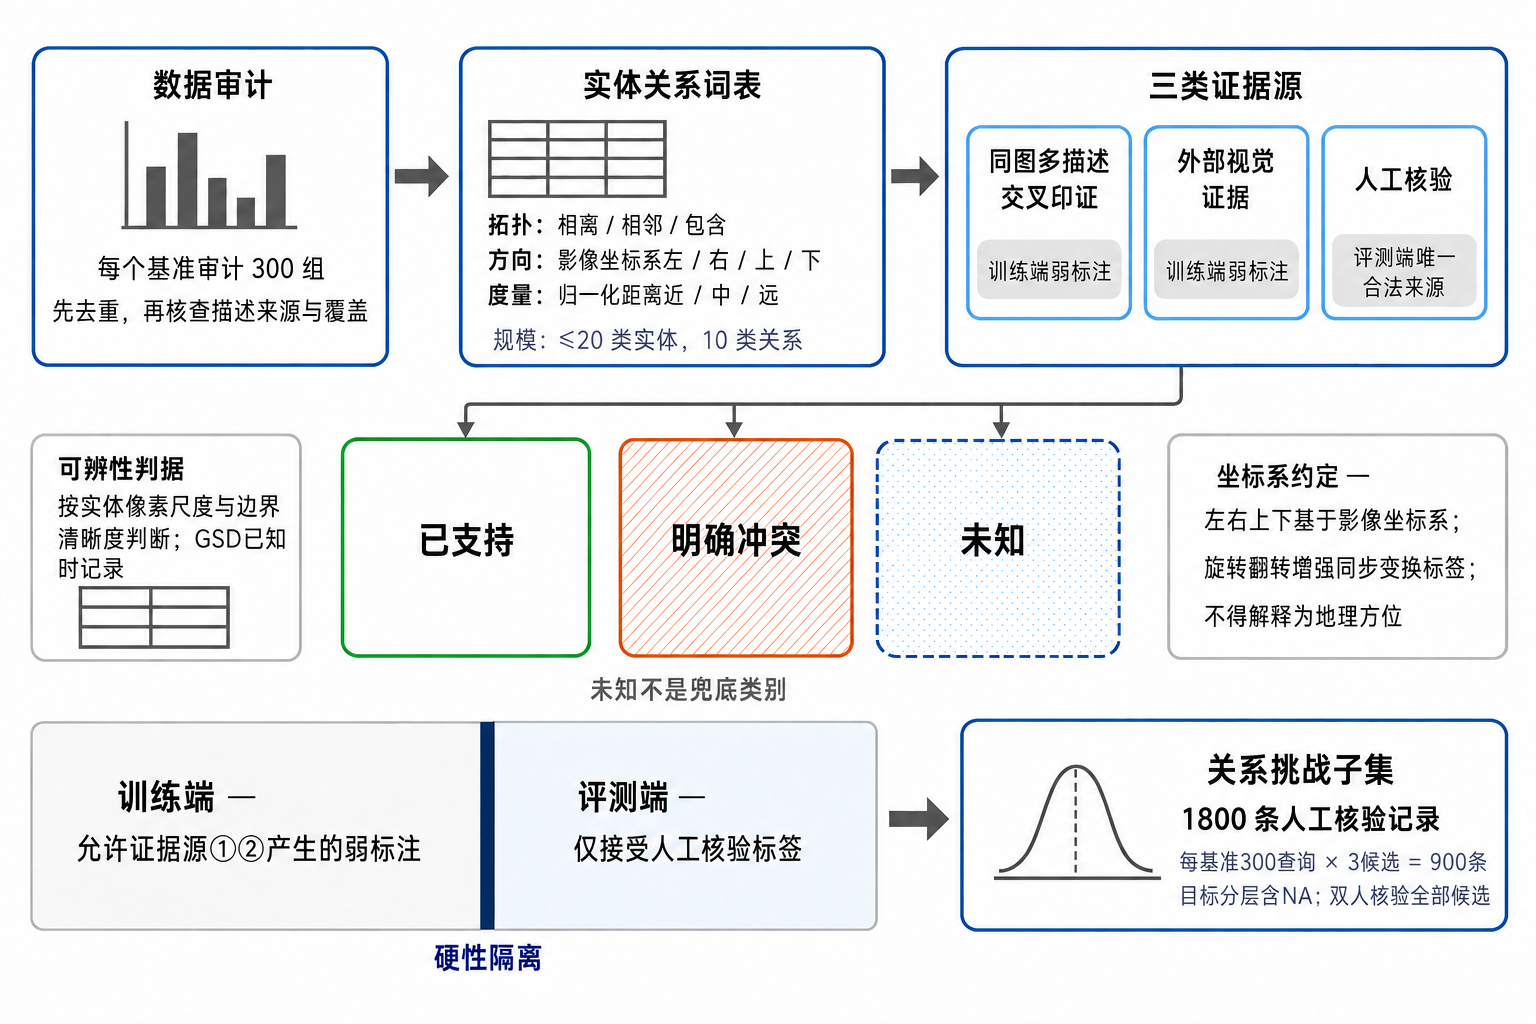
\includegraphics[width=\linewidth]{figures/F05_技术路线一-v3.png}
    \caption{技术路线一：关系证据三态建模。每个基准审计 300 组，先核查重复及描述来源；1800 条挑战记录覆盖固定候选组内全部查询—影像命题。}
    \label{fig:route-one}
\end{figure}


首先开展\textbf{公开数据审计}：在 RSITMD 与 RSICD 原始验证划分中，按场景类别比例各抽取\textbf{300 组、合计 600 组}影像及其全部配对描述，名义上为 3000 条记录。先保留原始索引，完成完全重复、近义改写和来源核对，再记录有效描述数、实体与关系、遗漏、矛盾及抽样种子。复制句和同源改写不增加支持票数；无法确认来源独立性的描述只作为多表述线索。审计样本用于开发规则和 H1 检验，与最终挑战影像隔离，原始训练、验证与测试划分保持不变。

其次\textbf{构建实体关系词表}：实体归并上限为\textbf{20 类}；候选关系最多\textbf{10 类}，包括相离、相邻、包含，影像坐标系的左、右、上、下，以及归一化距离近、中、远。距离以实体质心间距除以影像对角线长度，初始边界为 $1/3$ 和 $2/3$，边界误差超过定位精度时记为未知。RSICD 原始描述回避部分方向词\cite{lu2018rsicd}，因此不预设各类型均有充足自然样本。100 条开发试标后保留可稳定判定的关系，2027 年 1 月形成规范 v1，4 月完成开发期修订后冻结最终版本。

再次\textbf{建立三态判定规范}。标签绑定到具体 $(I,e_1,r,e_2)$：$I$ 是待判影像，$e_1,e_2$ 是命题限定的实体，$r$ 是所询问的关系。影像能够支持命题时标为 S（已支持），能可靠否定命题时标为 C（明确冲突），证据不足时标为 U（未知）。多实例且无法唯一指认、实体不可定位、分辨率不足或证据矛盾不能仲裁，均标 U；只有影像范围和精度足以可靠否定命题或所需实体存在时才标 C；仅未在描述中提及，不构成 C。记录实体指认依据、像素坐标、证据来源与判定理由。三类证据的作用如下：

\begin{enumerate}
    \item 同图描述（训练端弱线索）：RSICD 的复制补齐记录不能视为独立证据\cite{lu2018rsicd}，RSITMD 同样先核对文本与来源\cite{yuan2022amfmn}。只有去重后且来源可区分的描述共同提及同一命题，才记为弱支持候选；来源不明时不按独立票数提升置信度。互斥描述只生成待核查命题，必须由视觉证据确定哪一个命题被否定；文本矛盾本身不直接生成 C 标签。
    \item 视觉证据（训练端弱标注）：开放词汇检测或分割模型仅用于定位实体，再按预定的重叠、相对位置与距离规则判断关系。记录模型、训练来源及定位置信度，优先采用与检索编码器不同的骨干；来源无法核实的独立性不作保证。仅在定位和几何判定均可靠时生成弱 S 或弱 C，否则记 U。自动视觉证据不作为最终评测真值。
    \item 人工核验（评测标签来源）：1800 条候选命题全部由两人盲于模型输出、独立对照影像判断，形成 3600 次判定。先以验证集的 100 条记录试标并修订规范，正式标注前冻结版本；仲裁前报告三态 Cohen's $\kappa$，目标为 $\kappa\geq0.70$，并分关系组报告。申请人主持仲裁，随机复核 180 条记录，保留分歧和修改日志。完成的测试标签由评测人员封存，方法开发人员在最终配置冻结前不接触标签或测试分数。
\end{enumerate}

评测中的 S、C、U 均针对上述具体命题，不能把“两个文本来源不一致”替代“命题被影像否定”。有地面采样距离时记录其分档，缺失时记录像素尺度与可见性，不推断实际米制距离。对不可辨识的命题保留 U，以显示数据的判定边界。

此外还有一条必须固定的技术约定：左右、上下等相对关系一律基于影像坐标系定义，训练中的旋转与翻转增强必须同步变换相应关系标签；影像内的相对位置不得直接解释为地理方位。 三类证据源、记录字段与未知态判据见图~\ref{fig:evidence-sources}。

% F8: F08_三类证据源与适用边界-v2.png
\begin{figure}[!htb]
    \centering
    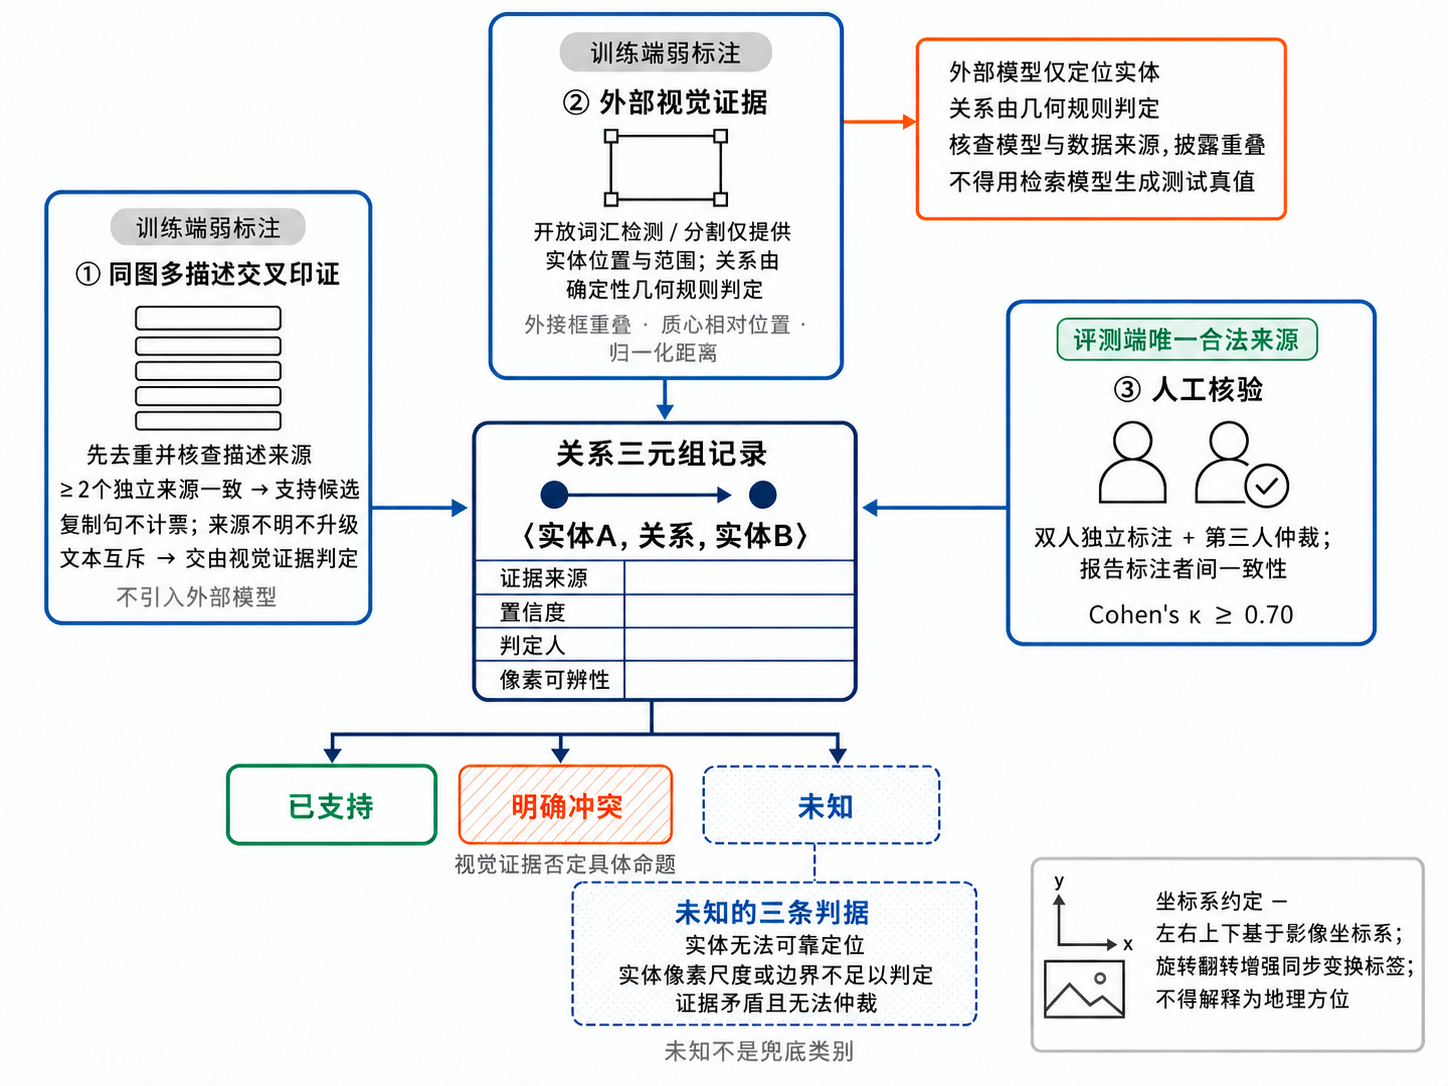
\includegraphics[width=\linewidth]{figures/F08_三类证据源与适用边界-v2.png}
    \caption{三态判定的证据来源与适用边界。外部模型仅定位实体，关系由几何规则判定；评测标签全部经人工核验。}
    \label{fig:evidence-sources}
\end{figure}


最后\textbf{分离开发与最终评测}：训练端使用弱标注，验证审计和试标用于规则修订；最终挑战集只使用人工影像核验标签，且不参与模型选择、阈值设置或规范修订。

关系挑战集的标注预算固定为\textbf{1800 条“候选影像—查询—目标关系命题”记录}，两基准各 900 条。每基准从原始测试集选择 300 幅经联合去重的影像，按场景类别和预先固定的基线特征组成 100 个互不重叠的三图候选组。每图从去重描述中按固定优先级选择一个明确关系命题，保留原句并抽取单关系查询，不添加原句未表达的关系。每个查询仅在同组 3 幅影像中排序，故每基准为 $300\times3=900$ 条候选命题；包括两个非原配候选在内全部核验，无需随模型返回结果追加标签。600 幅挑战影像与验证审计影像隔离，候选组和查询在测试前固定。此设计检验固定候选组内的关系区分，不能解释为全图库冲突发生率。

覆盖分层以查询原配影像的去重描述为依据：实际输入的单关系查询明确包含的实体和目标关系条目数，除以同图有效描述经核验合并后的条目数，得到\textbf{文本内部相对覆盖度}；低、中、高边界为 $1/3$、$2/3$。它不估计影像真实语义覆盖。只有一条有效描述、不同表述的条目集完全相同或分母为空者标为 NA，单独报告。每基准按三类关系各 100 个查询设初始配额，组内依据开发审计所得低、中、高及 NA 比例分配名额；具体整数名额、层内抽样种子和命题选择优先级在正式抽样前冻结。三类关系与低、中、高形成九格，另列 NA；若某格不足，先将余额按可用查询数分配至同关系组的其他覆盖层，再分配至其他可用关系组。按上述规则冻结样本清单，公布每格的实际数量、NA 比例及调整原因，不复制记录补额；总量仍不足时报告实际规模及功效限制。开发试标阶段进行功效敏感性分析，最终分层结果按实际区间宽度解释。

本内容形成的交付物为：覆盖 600 组影像的数据审计报告 1 份、实体关系词表与证据字段及判定规范各 1 套、1800 条人工核验关系挑战记录，以及双人标注、一致性统计、仲裁和抽查日志。

\subsubsection*{2.2.2\quad 内容二：兼顾关系判别与未知信息的跨模态匹配}

本内容回答“三态信息以何种方式进入目标函数才有效”。 共享骨干下的三臂对照及候选实现方式见图~\ref{fig:route-two}。

% F6: F06_技术路线二-v3.png
\begin{figure}[!htbp]
    \centering
    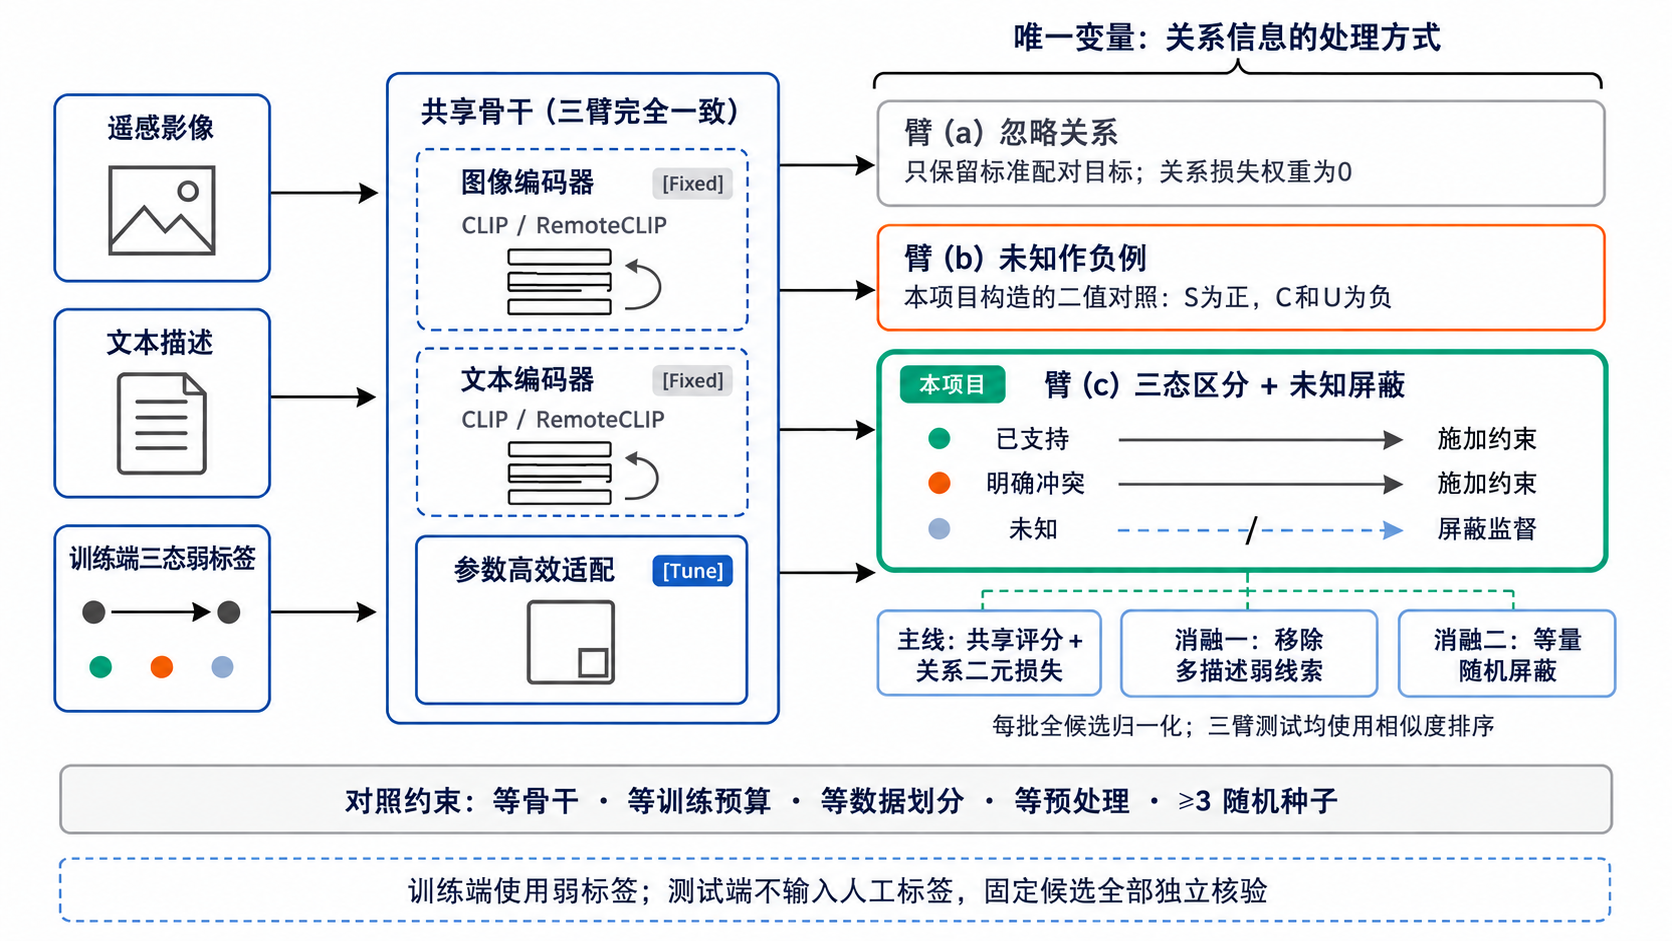
\includegraphics[width=\linewidth]{figures/F06_技术路线二-v3.png}
    \caption{技术路线二：三臂对照的关系约束匹配。三臂保持骨干、训练预算与数据设置一致，仅改变关系信息的处理方式。}
    \label{fig:route-two}
\end{figure}


以已有视觉语言编码器\cite{radford2021clip,liu2024remoteclip}为起点，采用参数高效适配\cite{yuan2023peft,zhou2022cocoop}控制规模。主线采用共享图文评分函数的关系监督：在标准图文对齐损失上增加关系命题的二元损失，S 为正例、C 为负例，U 的处理构成实验变量。三个处理臂共享骨干、适配器、评分函数与训练预算：

\begin{enumerate}
    \item 臂 (a)：关系损失权重为 0，只训练标准图文对齐目标；
    \item 臂 (b)：S 为正例，C 与 U 均作为关系负例；这是本项目构造的二值处理对照，不声称等价于 PMPGuard 或其他完整方法；
    \item 臂 (c)：S 为正例、C 为负例，U 的关系损失权重为 0。三个臂保留相同的标准配对目标，未知屏蔽仅作用于附加的关系监督。
\end{enumerate}

具体地，令 $p(I,\rho)=\operatorname{sigmoid}(s(I,\rho)/\tau+b)$，其中 $s$ 为共享编码器的相似度，$\rho$ 为完整关系命题文本。每批从训练描述抽取命题，并按固定规则为其选取原配影像和同场景非配影像构成候选集合；三臂使用相同集合，弱证据达不到判定条件者记 U，并报告 U 比例。关系损失使用二元交叉熵，按每批全部候选数归一化；臂 (c) 的 U 项置零，避免屏蔽后重加权扩大剩余样本作用。温度 $\tau>0$、偏置 $b$ 及关系权重在开发验证中统一选定并冻结；三臂共用温度与偏置，臂 (b)、(c) 及消融共用关系权重，臂 (a) 仍置零。三臂参数规模一致；测试统一使用图文相似度排序，不输入人工标签。12 次正式消融分别检验移除多描述弱线索，以及等量随机屏蔽的影响，每项在两基准各运行 3 个种子。随机屏蔽对照沿用臂 (b) 的目标标签，在每批全部候选中随机屏蔽与 U 同样数量的条目，沿用相同分母及固定随机种子；与臂 (c) 比较，以区分按证据状态屏蔽和一般减弱监督的作用。重排序或局部匹配只作为开发期主线失败时的备选，不再并列承诺额外正式实验。

证据置信度可借鉴已有不确定性建模\cite{chun2021pcme,han2021tmc,li2023pau,qin2022decl}，但本项目的标签对象固定为具体关系命题。弱标签的置信度阈值在开发阶段确定，最终评测仍以人工三态标签为准。

本内容形成的交付物为：核心方法、训练与推理代码、三臂对照与消融结果。

\subsubsection*{2.2.3\quad 内容三：标准检索与关系挑战的联合验证}

本内容回答“改进如何被归因到关系建模本身”。 联合验证与可归因性控制流程见图~\ref{fig:route-three}。

% F7: F07_技术路线三-v2.png
\begin{figure}[!htbp]
    \centering
    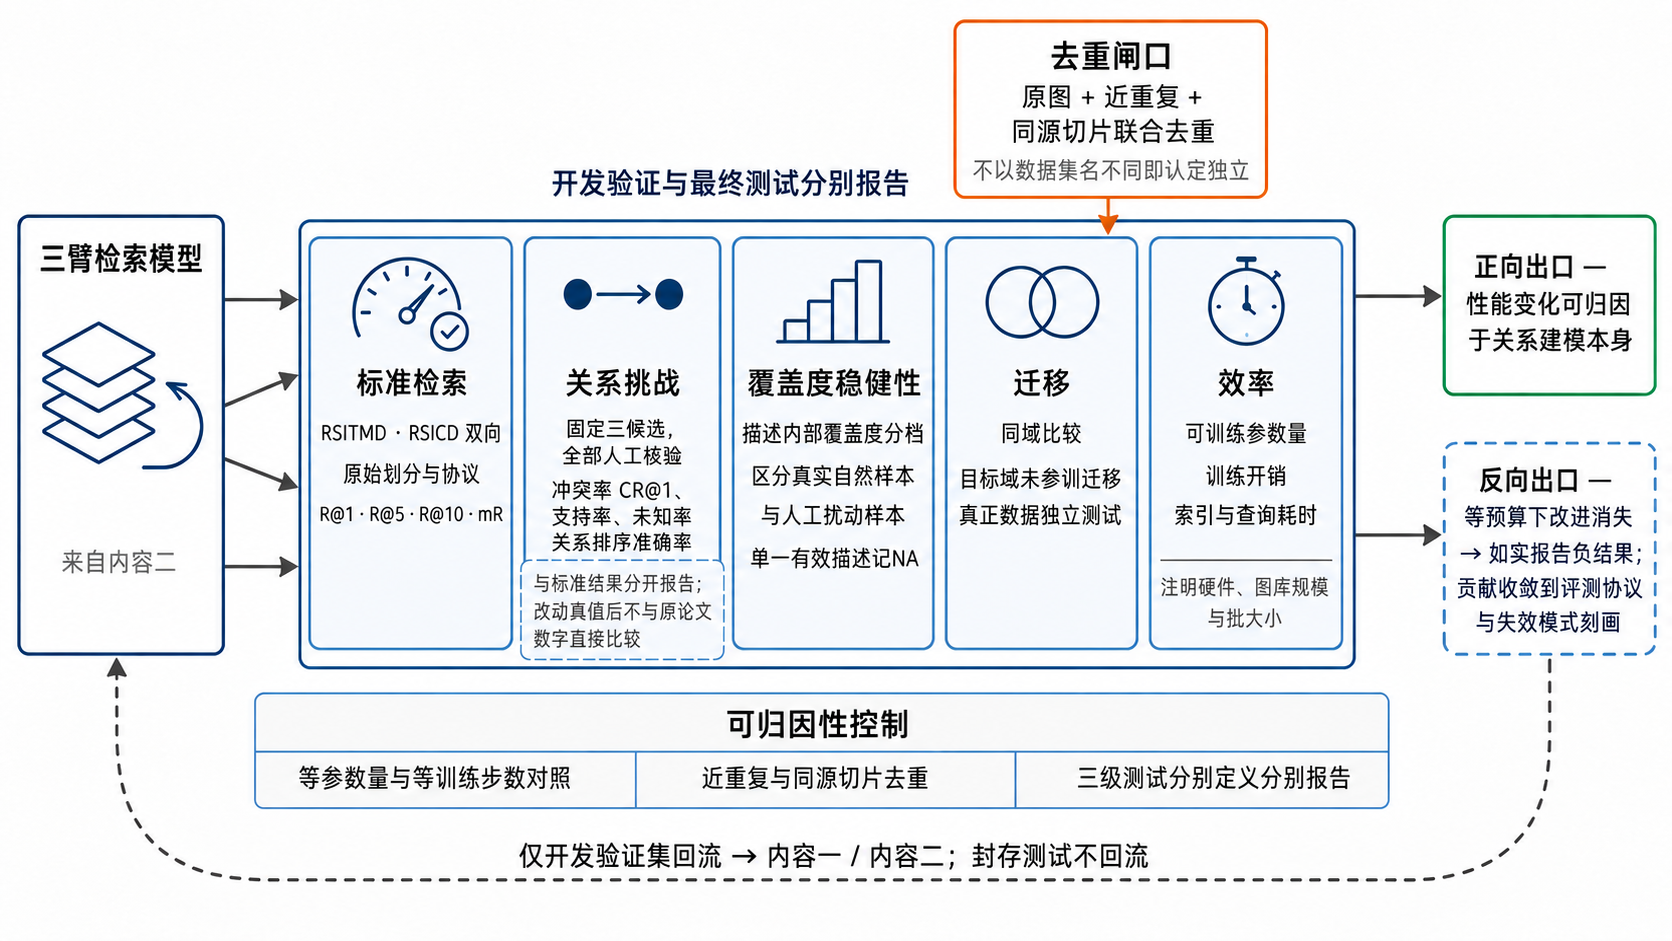
\includegraphics[width=\linewidth]{figures/F07_技术路线三-v2.png}
    \caption{技术路线三：联合验证。标准检索沿用原协议；关系挑战使用三图候选组。开发误差可回流，最终测试只用于冻结方案的检验。}
    \label{fig:route-three}
\end{figure}


\textbf{标准检索}沿用 RSITMD\cite{yuan2022amfmn} 与 RSICD\cite{lu2018rsicd} 的原始双向协议，分别报告 R@1、R@5 和 R@10，以六项均值作为 mR。挑战标签不改写标准配对真值。

\textbf{关系挑战}采用文本到影像的三图候选组，评价 top-1 排序。每个查询只含一个目标关系命题；原句含多关系时按预定优先级选一条，避免混合汇总不同命题的真值。得分相同的候选按固定影像索引排序。

\textbf{关系冲突误匹配率}记为 CR@1，\textbf{支持返回率}记为 SR@1。令 $Q$ 为全部挑战查询，$i_q^*$ 为查询 $q$ 的组内最高分候选，$y_{q,i}$ 为人工三态标签，则
\[
 \mathrm{CR@1}=\frac{\sum_{q\in Q}\mathbf{1}[y_{q,i_q^*}=C]}{|Q|},\qquad
 \mathrm{SR@1}=\frac{\sum_{q\in Q}\mathbf{1}[y_{q,i_q^*}=S]}{|Q|}.
\]
未知返回率 $\mathrm{UR@1}$ 同理以 U 计数，三率之和为 1，均以全部查询为分母。U 不当作正确或冲突，也不从分母中删去。H2 除要求 CR@1 降低外，还要求 SR@1 不降低且 UR@1 不增加；同时报告从冲突转为支持或未知的查询数量，区分正确返回与回避判定。

\textbf{关系排序准确率}比较同一查询中 S 候选与 C 候选的得分：S 得分较高计 1、相等计 $1/2$、较低计 0，总分除以全部可比较的 S--C 候选对数。U 不进入该分母；没有可比较对时记为 NA，同时报告有效查询数与候选对数。例如一组标签为 S、C、U，若返回 U，则 CR@1 为 0、UR@1 为 1、SR@1 为 0；只有 S 高于 C 才计一次关系排序正确。两基准分别报告并按查询合并，不将固定组的结果外推为全库指标。\textbf{覆盖度稳健性}按低、中、高及 NA 分层，真实描述与人工扰动结果分开报告。

\textbf{可归因性控制}是本内容的重点。包括三项措施：等参数量与等训练步数对照，用于排除容量与预算解释；跨数据集迁移前对原图、近重复影像与同源切片联合去重，不以数据集名称不同就认定相互独立；同域比较、目标域未参与训练的迁移测试、真正数据独立的测试三者分别定义并分别报告。这一要求有直接的现实依据：已有代表性遥感视觉语言模型在训练中使用了与检索基准相关的数据\cite{liu2024remoteclip}，若不加区分地报告，容易把数据重叠带来的收益误读为泛化能力。此外还需报告\textbf{效率指标}：可训练参数量、训练开销、索引与查询耗时，并注明硬件、图库规模与批大小。

本内容形成的交付物为：评测协议、分层结果报告、轻量检索演示与复现材料。

\subsection*{2.3\quad 三项内容的独立价值与相互关系}

三项内容分别形成数据规范、匹配方法和评测协议，其执行相互依赖，产出可分别检验与交付。

内容一产出的实体关系词表、三态判定规范与经人工核验的关系挑战子集，是\textbf{可独立发布的领域资源}：任何研究关系敏感检索、组合泛化或空间语义理解的工作都可直接使用，其价值不依赖于本项目内容二的方法是否成功。内容三产出的分层评测协议同样具有独立性——近重复去重、同域与迁移分别报告、等预算对照这套要求，可用于检验该方向\textbf{其它方法}的结论可归因性，是对领域评测规范的贡献。内容二则是在前两者支撑下对核心假说的直接检验。

内容二即使未获得预期性能，数据规范与对照评测仍可形成研究结果。两次规则及方法回流仅使用验证集审计、试标和开发实验，分别安排在 2027 年 1 月和 4 月；最终测试保持封存，不参与闭环修订。

\subsection*{2.4\quad 拟解决的关键科学问题}

本项目拟解决的关键科学问题是：\textbf{在遥感图文数据中文本描述对影像内容的覆盖天然不完备的条件下，如何在跨模态匹配中区分“描述未覆盖”与“实际关系冲突”，使有证据的地理实体关系参与约束、而不可判定的关系不被当作监督信号？}

检验重点是证据状态与监督效果之间的关系：何种命题可以稳定判定，未知屏蔽在什么条件下有效，以及观察到的差异能否排除容量和预算解释。三项研究内容分别提供其数据、方法与验证依据。


\CasmTopic{3. 拟采取的研究方案及可行性分析}{（包括研究方法、技术路线、实验手段、关键技术等说明）}

% 内容来源：NSFC_2027_Mapping/extraTex/2.1.研究内容.tex
\subsection*{3.1\quad 研究方法}

本项目采用数据审计、受控对照与独立测试相结合的方法。两次开发回流完成后，于 2027 年 4 月底冻结标注规范、查询与候选组、模型结构、超参数选择规则和评价脚本。正式实验在两基准分别使用种子 2026、2027、2028：三臂共 18 次主实验，两项消融共 12 次，合计 30 次。模型选择只使用训练和验证数据；全部检查点选定后，最终测试由评测人员一次性批量运行，后续错误分析仅用于结果解释。

报告三种子的均值、标准差与各次结果。对方法差值进行 2000 次配对 bootstrap：关系挑战以不重叠三图组为重采样单位、按基准分层，标准检索以影像及其全部配对描述为聚类单位，在固定全库排名上重采样；各次保留三个种子的配对结果并取均值，给出 95\% 置信区间。H2 的联合判据为臂 (c) 减臂 (b) 的 CR@1 差值区间上限小于 0、SR@1 差值区间下限不低于 0、UR@1 差值区间上限不高于 0，且两个基准的标准 mR 差值区间下限均不低于 $-1$ 个百分点。有效比较不足或区间不满足判据时，报告证据不足；不以“不显著”解释为等效。上述区间反映固定三个种子下的测试样本不确定性，种子间变异另以标准差呈现。H3 结合相同参数与训练预算、消融及数据来源核对评估。

\subsection*{3.2\quad 技术路线}

技术路线按“数据审计、关系证据、匹配方法、联合验证”组织，开发期验证结果用于修订，最终测试只承担冻结方案的检验。

RSITMD 与 RSICD 经审计、去重后形成训练弱标签、验证审计记录和封存测试候选组；许可满足时，以少量 SkyScript\cite{wang2024skyscript} 数据补充验证。内容二在训练数据上实现三臂方法，内容三先用验证集检查失效模式。2027 年 1 月与 4 月各进行一次开发回流，随后冻结规范和配置；正式训练完成后一次性开展标准检索、关系挑战、覆盖度、迁移与效率测试。

若最终测试发现标注或程序错误，只按冻结规范进行与模型得分无关的更正，并保留原始结果、修订原因和受影响范围；测试反馈不用于重新选模型、调整阈值或修改关系定义。

\subsection*{3.3\quad 关键技术}

\begin{enumerate}
    \item 三态关系证据的判定与表示：在仅有图像级描述、缺少实体框与拓扑真值的条件下，定义可操作、可复核的三态判据，并处理坐标系依赖与几何增强的标签同步问题。这是本项目最核心也最容易被低估的技术难点。
    \item 未知态屏蔽的监督构造：在附加关系损失中实现未知屏蔽，同时避免因屏蔽过多而削弱训练信号；需要在屏蔽比例与训练稳定性之间找到可用区间。
    \item 弱标注与人工核验的协同使用：训练端容忍弱标注噪声、评测端坚持人工核验，二者的边界必须在流程上硬性隔离，防止弱标注污染测试集。
    \item 近重复去重与分层评测实施：对原图、近重复影像与同源切片进行有效识别，并保证同一影像的全部描述落在同一数据划分内。
\end{enumerate}

\subsection*{3.4\quad 可行性分析}

\textbf{理论可行性}：图像级描述只能提供部分语义，重复记录还会影响有效信息量\cite{lu2018rsicd,yuan2022amfmn}；已有工作已证明可以利用部分匹配中的有效线索和鲁棒学习处理失配\cite{pmpguard2026,hu2023rcl,han2023msc}。这些基础支持进一步检验具体关系命题的三态监督，但并不预先保证 H1--H3 成立。视觉语言编码器、参数高效适配与不确定性建模提供了可复用组件\cite{radford2021clip,liu2024remoteclip,yuan2023peft,chun2021pcme,li2023pau}。

\textbf{技术可行性}：三项内容均不依赖尚不存在的技术。内容一是标注规范与数据工程；内容二在成熟编码器上做受控改动，训练规模由参数高效适配控制；内容三是评测协议设计与实施。方法路线刻意避开了从零训练大模型这类高风险高成本路径。

\textbf{数据可行性}：RSITMD 与 RSICD 的公开获取入口已经核验，作者仓库提供影像、标注与解析程序；数据的实际获取与逐样本验证安排在启动阶段完成，其当前状态详见“研究基础与工作条件”第 1 小节的前期基础边界说明。

\textbf{条件可行性}：申请人在遥感影像空间结构理解与跨模态检索两个方向的积累恰好构成本项目所需的能力组合，并具备相应的算力与工程基础，详见“研究基础与工作条件”部分。

\textbf{风险可控性}：本项目为三条假说均预设了证伪条件与降级路径（详见本小节后文的研究风险与应对措施）。特别地，若启动阶段（2026 年 11 月至 2027 年 1 月）的错误归因表明“描述不完备”并非主要误差来源，本项目将据此调整内容一的定位乃至研究题目，而不会通过反向挑选样本维持既定结论。把退出路径写在方案里，本身就是可行性的一部分。

% 内容来源：NSFC_2027_Mapping/extraTex/3.1.研究基础.tex
\subsection*{3.5\quad 研究风险与应对措施}

本项目的主要风险及应对预案如下。所有预案均以“如实报告、调整定位”为原则，不通过改动评测口径或抽样方式维持既定结论。 三条假说的检验时点、证伪判据与降级路径见图~\ref{fig:falsification}。

% F11: F11_假说证伪-v3.png
\begin{figure}[!htbp]
    \centering
    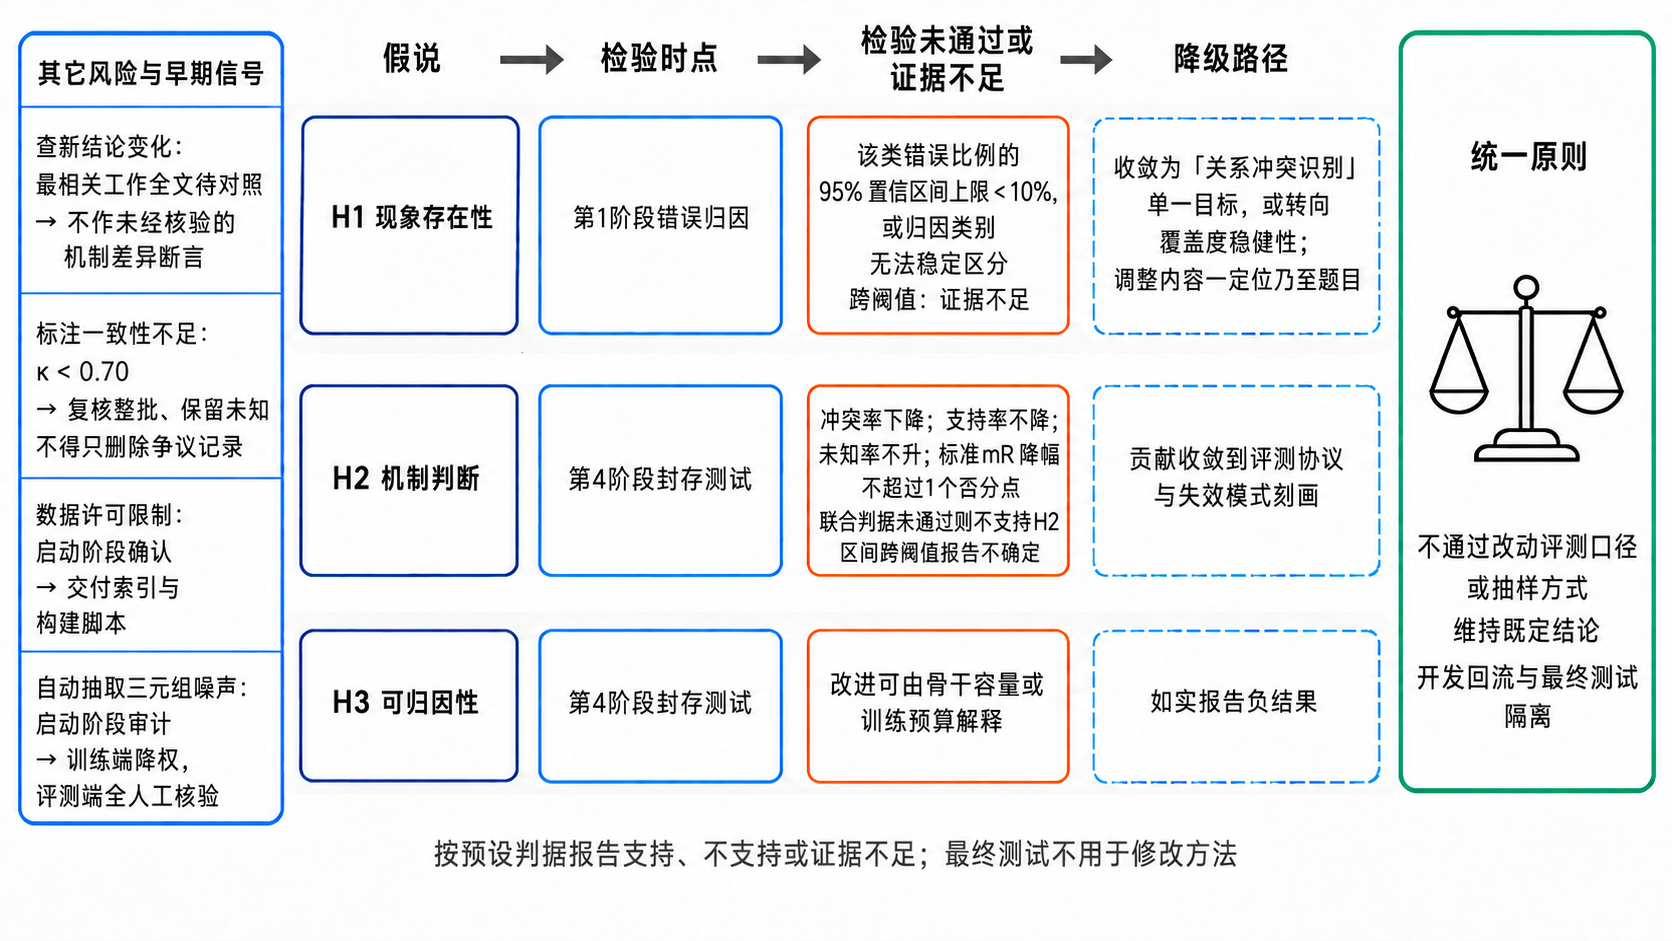
\includegraphics[width=\linewidth]{figures/F11_假说证伪-v3.png}
    \caption{假说、检验判据与调整路径。H1 继续投入阈值固定为 10\%，结合 95\% 置信区间判断；H2 同时要求支持返回率不降低、未知返回率不增加、标准 mR 降幅不超过 1 个百分点；标注一致性目标为 $\kappa \geq 0.70$。}
    \label{fig:falsification}
\end{figure}


\begin{enumerate}
    \item 科学假说未通过检验的风险。若启动阶段（2026 年 11 月至 2027 年 1 月）审计所得 H1 错误占比的 95\% 置信区间上限低于 10\%，或归因类别无法稳定区分，则不再将其作为项目的主要误差来源；区间跨越阈值时保留不确定结论。\textbf{应对}：收缩为关系冲突识别或覆盖度稳健性分析，继续完成既定的数据规范、独立评测和可复现研究成果，不反向修改阈值、抽样规则或真值标签。H2 或 H3 未得到支持时如实报告对照结果，以评测协议与失效模式分析形成论文和研究报告。

    \item 查新结论变化的风险。空间感知实体关系探索\cite{shui2025esrn}是最相关工作之一，目前全文尚未取得。\textbf{应对}：现阶段仅据可核验题录说明其研究主题，不据此认定其没有三态或未知态设计；取得全文后按标签对象、证据来源、监督方式和评测设计逐项比较。创新表述限于本项目拟研究的机制及验证安排，其相对新颖性仍需全文查新确认。

    \item 关系标注一致性或样本量不足的风险。\textbf{应对}：先在验证集完成 100 条试标，两次开发修订后冻结规范，再开展 1800 条正式标注；目标为仲裁前 $\kappa\geq0.70$。若正式一致性不足，按冻结规范复核整批受影响记录，保留各轮数值，不因测试效果修改定义或删除分歧记录。不可判定者保留 U；若缺乏足够关系查询或 S--C 对，依预定配额规则调整并报告实际规模及检验能力，不补造样本。

    \item 改进无法归因的风险。若性能提升可由骨干容量或训练预算解释，则本项目的机制主张不成立。\textbf{应对}：2027 年 5--7 月安排等参数量、等训练步数对照实验专门检验；若改进在等预算条件下消失，将如实报告负结果，并把贡献收敛到评测协议与失效模式刻画。

    \item 数据许可与进度风险。第三方数据许可可能不允许再分发影像或派生标注；参与研究生的分工与投入需按申报时点确认。\textbf{应对}：成果交付优先采用数据索引、处理脚本、版本说明与获准发布的派生内容，许可在启动阶段确认；三项内容虽有先后依赖但可并行推进，内容三的协议设计可与内容一、二同步开展，论文撰写安排在 2027 年 5--7 月启动，8--10 月完成 1 篇论文并投稿，审稿进度据实记录。
\end{enumerate}


\CasmTopic{4. 课题的特色与创新之处}{（包括主要特色和创新点等）}

% 内容来源：NSFC_2027_Mapping/extraTex/2.2.特色与创新.tex
\subsection*{4.1\quad 项目特色}

本项目首先审计关系监督的依据：对某个具体命题，描述遗漏、视觉冲突与视觉不可判定如何区分，各自会怎样影响训练。

已有细粒度对齐与关系增强提供了方法基础。本项目在共享编码器和固定训练预算下改变关系证据的使用方式，将性能差异与监督构造联系起来。

第二个特色是\textbf{预先规定可证伪判据}。多描述数据的有效信息量需先核查\cite{lu2018rsicd,yuan2022amfmn}，现有部分匹配与鲁棒学习也已能保留有效语义\cite{pmpguard2026,hu2023rcl}，因此本项目不预设新方法一定有效。H1 在启动后三个月内审计，H2--H3 在冻结方法后的独立测试中检验；证据不足时保留不确定或负结果。

第三个特色是\textbf{证据纪律}。训练端允许使用自动抽取的弱标注，评测端坚持人工核验；标准检索、关系挑战、迁移测试分别报告；改动过真值的评测绝不与原论文数字直接比较。这些约束会让最终报出来的数字更保守，换来的是结论可被他人复现与检验。

\subsection*{4.2\quad 创新点}

\begin{enumerate}
    \item 研究关系命题的可判定状态及其监督作用。在已有关系增强\cite{zhang2023unimodal,shui2025esrn,wu2024scat,yang2024dove,mi2024knowledgeaware}和失配处理\cite{hu2023rcl,han2023msc,yang2023bicro,zhang2024npc,feng2024tripartition,pmpguard2026}基础上，将标签绑定到具体影像和实体关系命题，显式保留 S、C、U，并用共享评分函数检验未知屏蔽的作用。拟贡献在于可复核的状态定义及其受控验证，不能以“既有方法均不区分成因”作为创新前提。

    \item 将描述覆盖差异与候选真值核验结合。去重和来源核对后的描述可提供训练弱线索，视觉及人工证据确定其适用边界；通过全候选核验的三图挑战组，同时报告冲突、支持与未知返回率，检验关系约束的收益是否真实。文本内部覆盖度与不可估计的 NA 分层分别报告，避免把描述数量或覆盖比值误解为完整影像真值。
\end{enumerate}

\subsection*{4.3\quad 与最相关工作的差异说明}

需要明确的是，空间关系增强与不完备图文对应\textbf{均已有成熟研究}，本项目不作任何“首次”或“填补空白”的主张。与最相关工作的差异如下：

PMPGuard\cite{pmpguard2026}既估计伪匹配程度，也通过注意力利用部分匹配中的正、负语义线索；本项目不能将其简化为统一抑制噪声。拟比较的重点是具体关系命题的三态标签、未知屏蔽位置及独立候选真值协议。实体关系单模态学习\cite{zhang2023unimodal}和 ESRN\cite{shui2025esrn}提供关系增强思路，其中 ESRN 当前仅核实题录，可靠摘要与全文均未取得，尚不能判断其与三态设计是否存在方法重叠。通用不确定性及证据学习\cite{chun2021pcme,han2021tmc,li2023pau,qin2022decl}可作为技术参照；本项目拟将其落实到可人工复核的关系命题。图~\ref{fig:positioning}仅归纳已核验的研究主题，不表示已完成全部方法查新。

% F9: F09_差异定位-v2.png
% 保持图文合排，避免前文重排后将留白转移到此图的独立插图页。
\begin{figure}[!htb]
    \centering
    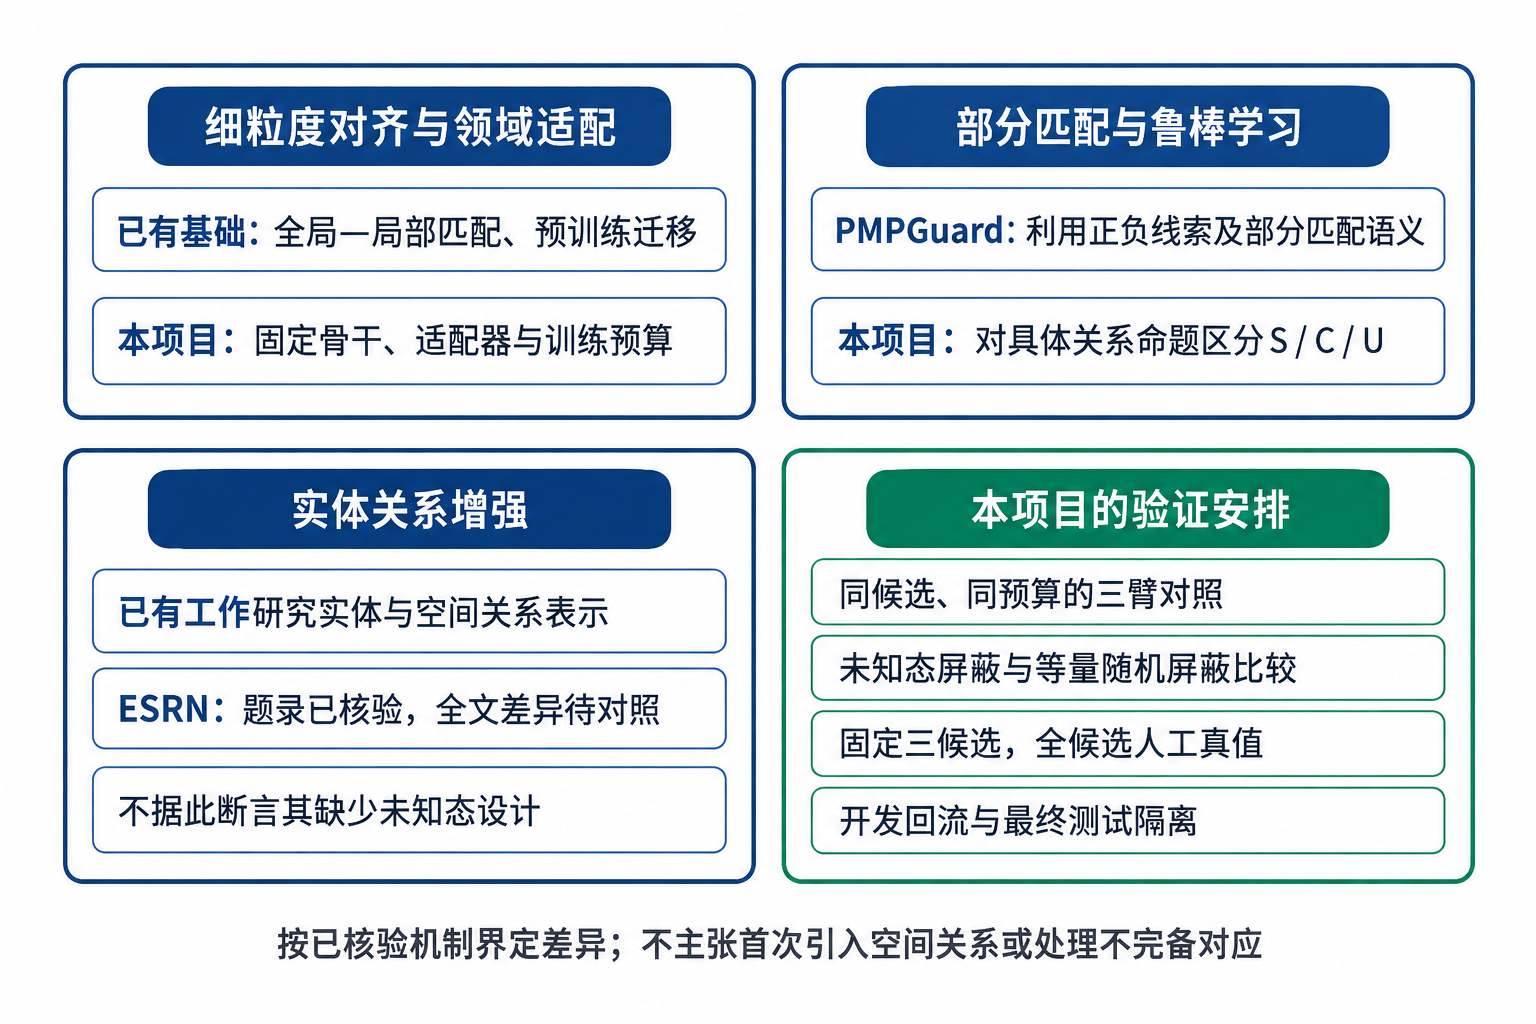
\includegraphics[width=\linewidth]{figures/F09_差异定位-v2.png}
    \caption{相关工作与拟研究重点。PMPGuard 利用部分匹配正、负线索；ESRN 仅据题录标示关系研究主题，其方法重叠仍待全文核查。}
    \label{fig:positioning}
\end{figure}


本项目的创新主张因此限定为：\textbf{把关系证据的可判定状态作为跨模态匹配中的一等建模对象，研究仅对可核验关系施加约束、对未知关系不施加监督的对齐方式，并用独立核验的关系证据检验其效果。}这是方法层面的问题重述与验证设计，不是新任务或新领域的开创性声明。


\CasmTopic{5. 年度研究计划及预期研究成果}{（包括研究计划、拟组织的重要学术交流活动、国际合作与交流计划、预期研究成果等）}

% 内容来源：NSFC_2027_Mapping/extraTex/2.3.年度研究计划.tex
\subsection*{5.1\quad 年度研究计划}

本项目执行期为 2026 年 11 月 1 日至 2027 年 10 月 31 日，共 1 年（12 个月）。围绕数据审计、主线方法与可归因性验证，按四个连续阶段组织研究。年度任务固定为：600 组数据审计、1800 条挑战记录双人标注、18 次三臂主实验、12 次关键消融、五类评测报告，以及 1 篇论文投稿和代码、演示、结题报告交付。各阶段按下述数量与期限推进，研究结论依据实际数据形成；一年任务安排与 H1 检验节点见图~\ref{fig:timeline}。

% F10: F10_年度研究计划-v2.png
\begin{figure}[!htbp]
    \centering
    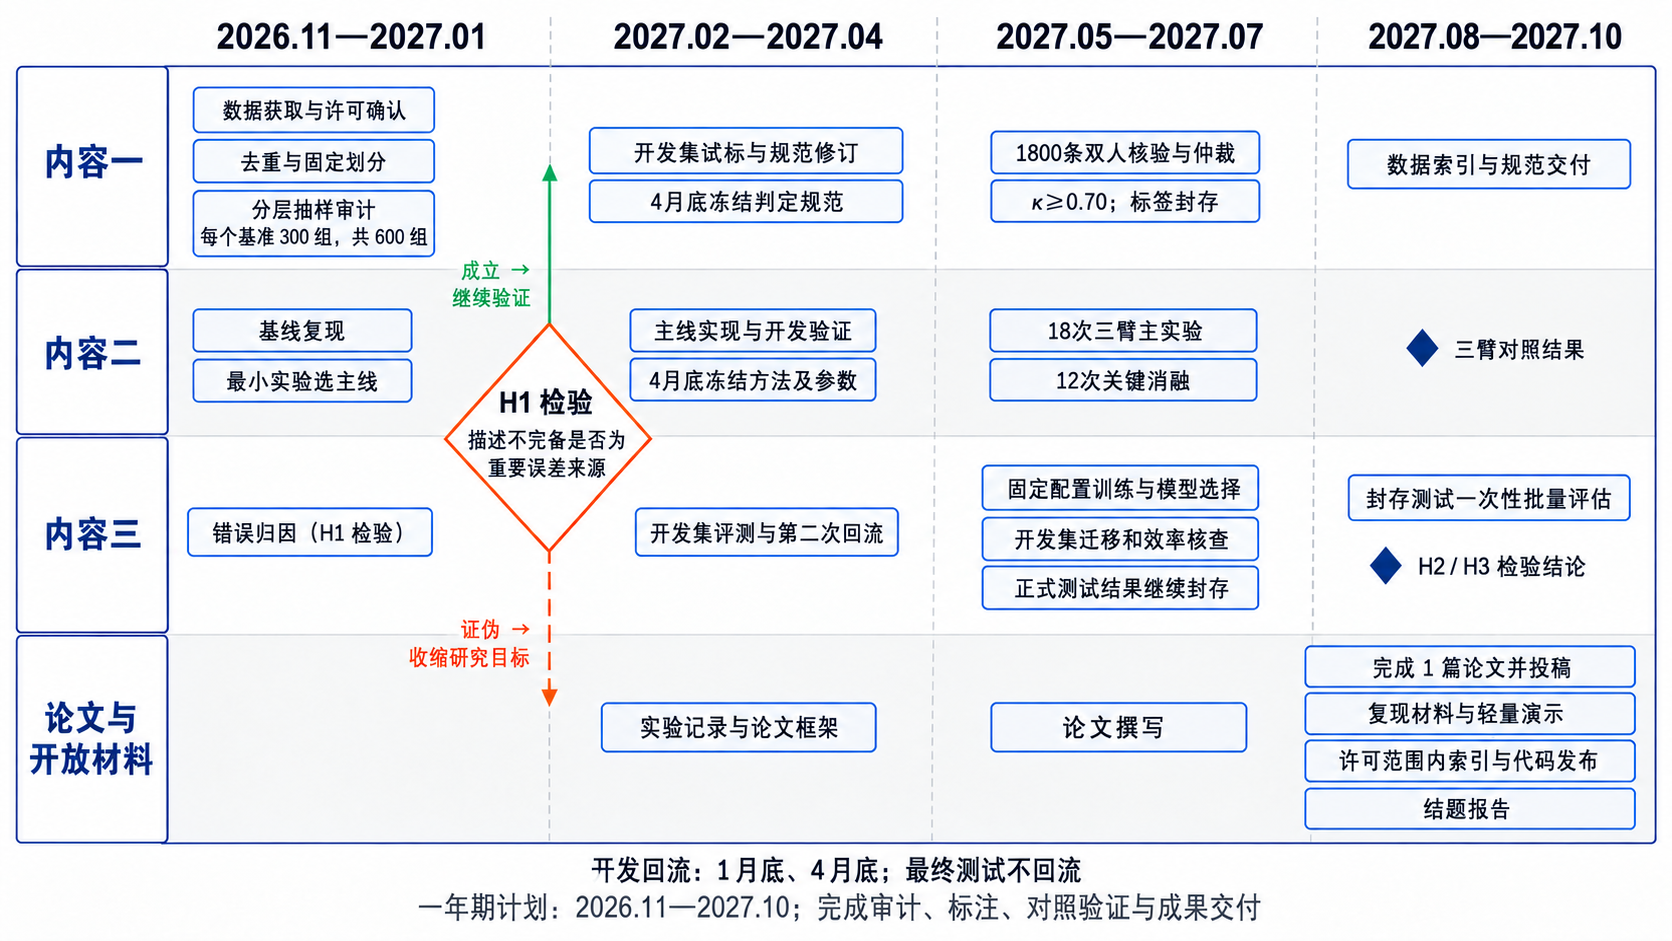
\includegraphics[width=\linewidth]{figures/F10_年度研究计划-v2.png}
    \caption{一年期研究计划与里程碑。执行期为 2026.11--2027.10，分四个阶段推进，H1 检验在 2027 年 1 月底前完成；阶段任务与交付物以本节说明为准。}
    \label{fig:timeline}
\end{figure}

\subsubsection*{5.1.1\quad 第一阶段（2026.11--2027.01）：数据基础与假说检验}

本阶段的核心任务是\textbf{检验假说 H1}，审计描述遗漏相关现象是否达到预设的研究取舍阈值，为后续方法研究确定边界。

完成 RSITMD、RSICD 的获取、许可和完整性核对，检查原图、近重复影像及同源切片，保持官方划分。从验证集各抽取 300 组影像，审计其名义 3000 条描述记录并统计去重后的有效信息量；复现 CLIP\cite{radford2021clip}、RemoteCLIP\cite{liu2024remoteclip}及参数高效适配\cite{yuan2023peft}基线，完成 H1 审计与区间分析。形成最多 20 类实体、10 类关系的规范草案，完成 100 条试标和第一次开发回流，确定关系监督主线；测试标签与分数不用于调参。

\textbf{阶段目标}：2027 年 1 月底前交付 600 组审计、基线与 H1 报告、去重及描述来源记录、规范 v1、100 条试标报告，预先确定挑战集抽样、NA 与配额调整规则。

\subsubsection*{5.1.2\quad 第二阶段（2027.02--2027.04）：关系挑战子集与方法实现}

根据开发实验完成第二次回流，4 月底冻结关系规范、方法配置及评价脚本。评测人员按固定规则选取每基准 100 个三图候选组、完成挑战查询和样本清单，开始双人独立核验；方法人员完成三臂训练代码及验证集检查，形成中期记录和论文框架。标签封存管理与方法开发分工实施。

\textbf{阶段目标}：2027 年 4 月底前交付冻结的规范、候选组与分层清单、训练及评测代码和中期记录；计划 1800 条、3600 次正式判定在后续最终测试前完成，保留一致性、仲裁及抽查报告。

\subsubsection*{5.1.3\quad 第三阶段（2027.05--2027.07）：可归因性验证与论文撰写}

在冻结配置下完成两基准各三臂、三种子的 18 次主实验，以及两项消融各两基准、三种子的 12 次实验；全部检查点仅依据验证集选定。完成 1800 条挑战记录的双人核验、仲裁及 180 条抽查，封存标签和一致性报告。以验证结果开展五类分析、检查两个方向的迁移流程，并形成论文初稿；H2--H3 的最终结论留待独立测试。

\textbf{阶段目标}：2027 年 7 月底前交付 30 次正式实验日志、固定检查点、挑战标签与质量报告、验证集五类分析，以及论文初稿；封存文件版本和哈希，准备独立测试。

\subsubsection*{5.1.4\quad 第四阶段（2027.08--2027.10）：独立复核、成果整理与结题}

评测人员对冻结的检查点、脚本和标签一次性运行最终测试，完成五类评测、2000 次聚类重采样与 H2--H3 判断。后续复核仅解释结果或按冻结规范纠正可追踪的错误，不再调参；成果于 2027 年 10 月底前整理交付。

\textbf{阶段目标}：完成 1 篇论文投稿，交付代码与复现材料、轻量演示、评测协议、关系规范、1800 条挑战记录和结题报告。数据按许可交付；原始影像不能公开时提供索引、构建脚本和获准发布的派生记录。

\subsection*{5.2\quad 学术交流安排}

2027 年 5--7 月安排 1 人次国内合作交流，讨论关系判定规范、实验设计或阶段结果，使用现有 0.50 万元差旅预算；具体行程按合作单位安排执行。日常技术讨论采用线上方式，不安排本项目经费支持的国际出访或会议主办。

\subsection*{5.3\quad 预期研究结果}

\subsubsection*{5.3.1\quad 学术成果}

完成\textbf{1 篇学术论文并于 2027 年 10 月底前投稿}，以稿件和投稿记录验收；接收与发表依实际评审进度，按要求标注资助信息。假说未得到支持时，据实报告对照结果和失效分析。

\subsubsection*{5.3.2\quad 方法与技术成果}

形成面向不完备描述的地理实体关系证据表示方法 1 套，包括实体关系词表、证据字段规范与三态判定规则；形成仅约束可核验关系、屏蔽未知态的跨模态匹配方法 1 套，含三臂对照与必要消融证据。

\subsubsection*{5.3.3\quad 数据与工具成果}

交付\textbf{1800 条}双人核验的挑战记录、\textbf{600 组}影像及全部描述的审计记录，附规范、索引和一致性报告；算法与评测代码、复现材料、轻量演示各 1 套，附环境、划分、模型来源、种子和日志，以及五类评测报告和结题报告。原始影像不再分发，数据成果按许可交付。

\subsubsection*{5.3.4\quad 人才培养}

组织成员表中的 7 名新疆大学研究生按既定分工接受科研训练，不承诺一年内完成学位培养。劳务费按 2 个集中助研岗位、各 6 个月测算，人员、投入月份和发放依据按阶段任务据实核定。

\subsubsection*{5.3.5\quad 关于成果表述的说明}

上述数量为执行期计划，按实际记录验收；假说按预设判据判断，据实报告样本不足、不确定性与负结果。
